\documentclass[twoside]{book}

% Packages required by doxygen
\usepackage{calc}
\usepackage{doxygen}
\usepackage{graphicx}
\usepackage[utf8]{inputenc}
\usepackage{makeidx}
\usepackage{multicol}
\usepackage{multirow}
\usepackage{textcomp}
\usepackage[table]{xcolor}

% Font selection
\usepackage[T1]{fontenc}
\usepackage{mathptmx}
\usepackage[scaled=.90]{helvet}
\usepackage{courier}
\usepackage{amssymb}
\usepackage{sectsty}
\renewcommand{\familydefault}{\sfdefault}
\allsectionsfont{%
  \fontseries{bc}\selectfont%
  \color{darkgray}%
}
\renewcommand{\DoxyLabelFont}{%
  \fontseries{bc}\selectfont%
  \color{darkgray}%
}

% Page & text layout
\usepackage{geometry}
\geometry{%
  a4paper,%
  top=2.5cm,%
  bottom=2.5cm,%
  left=2.5cm,%
  right=2.5cm%
}
\tolerance=750
\hfuzz=15pt
\hbadness=750
\setlength{\emergencystretch}{15pt}
\setlength{\parindent}{0cm}
\setlength{\parskip}{0.2cm}
\makeatletter
\renewcommand{\paragraph}{%
  \@startsection{paragraph}{4}{0ex}{-1.0ex}{1.0ex}{%
    \normalfont\normalsize\bfseries\SS@parafont%
  }%
}
\renewcommand{\subparagraph}{%
  \@startsection{subparagraph}{5}{0ex}{-1.0ex}{1.0ex}{%
    \normalfont\normalsize\bfseries\SS@subparafont%
  }%
}
\makeatother

% Headers & footers
\usepackage{fancyhdr}
\pagestyle{fancyplain}
\fancyhead[LE]{\fancyplain{}{\bfseries\thepage}}
\fancyhead[CE]{\fancyplain{}{}}
\fancyhead[RE]{\fancyplain{}{\bfseries\leftmark}}
\fancyhead[LO]{\fancyplain{}{\bfseries\rightmark}}
\fancyhead[CO]{\fancyplain{}{}}
\fancyhead[RO]{\fancyplain{}{\bfseries\thepage}}
\fancyfoot[LE]{\fancyplain{}{}}
\fancyfoot[CE]{\fancyplain{}{}}
\fancyfoot[RE]{\fancyplain{}{\bfseries\scriptsize Generated on Thu Jun 16 2016 12\-:06\-:08 for e-\/\-Meter by Doxygen }}
\fancyfoot[LO]{\fancyplain{}{\bfseries\scriptsize Generated on Thu Jun 16 2016 12\-:06\-:08 for e-\/\-Meter by Doxygen }}
\fancyfoot[CO]{\fancyplain{}{}}
\fancyfoot[RO]{\fancyplain{}{}}
\renewcommand{\footrulewidth}{0.4pt}
\renewcommand{\chaptermark}[1]{%
  \markboth{#1}{}%
}
\renewcommand{\sectionmark}[1]{%
  \markright{\thesection\ #1}%
}

% Indices & bibliography
\usepackage{natbib}
\usepackage[titles]{tocloft}
\setcounter{tocdepth}{3}
\setcounter{secnumdepth}{5}
\makeindex

% Hyperlinks (required, but should be loaded last)
\usepackage{ifpdf}
\ifpdf
  \usepackage[pdftex,pagebackref=true]{hyperref}
\else
  \usepackage[ps2pdf,pagebackref=true]{hyperref}
\fi
\hypersetup{%
  colorlinks=true,%
  linkcolor=blue,%
  citecolor=blue,%
  unicode%
}

% Custom commands
\newcommand{\clearemptydoublepage}{%
  \newpage{\pagestyle{empty}\cleardoublepage}%
}


%===== C O N T E N T S =====

\begin{document}

% Titlepage & ToC
\hypersetup{pageanchor=false}
\pagenumbering{roman}
\begin{titlepage}
\vspace*{7cm}
\begin{center}%
{\Large e-\/\-Meter \\[1ex]\large 0.\-1 }\\
\vspace*{1cm}
{\large Generated by Doxygen 1.8.6}\\
\vspace*{0.5cm}
{\small Thu Jun 16 2016 12:06:08}\\
\end{center}
\end{titlepage}
\clearemptydoublepage
\tableofcontents
\clearemptydoublepage
\pagenumbering{arabic}
\hypersetup{pageanchor=true}

%--- Begin generated contents ---
\chapter{Hierarchical Index}
\section{Class Hierarchy}
This inheritance list is sorted roughly, but not completely, alphabetically\-:\begin{DoxyCompactList}
\item \contentsline{section}{Client\-Socket}{\pageref{classClientSocket}}{}
\item \contentsline{section}{cs5463\-Commands}{\pageref{structcs5463Commands}}{}
\item \contentsline{section}{cs5463\-Electricity\-Attr}{\pageref{structcs5463ElectricityAttr}}{}
\item \contentsline{section}{cs5463\-Reg\-Add\-Pg1}{\pageref{structcs5463RegAddPg1}}{}
\item \contentsline{section}{cs5463spi\-Params}{\pageref{structcs5463spiParams}}{}
\item \contentsline{section}{cs5463sys\-Cal\-Gain\-Vals}{\pageref{structcs5463sysCalGainVals}}{}
\item \contentsline{section}{cs5463sys\-Cal\-Offset\-Vals}{\pageref{structcs5463sysCalOffsetVals}}{}
\item \contentsline{section}{Logger}{\pageref{classLogger}}{}
\item \contentsline{section}{logger\-Info}{\pageref{structloggerInfo}}{}
\item \contentsline{section}{Reg\-Read\-Cmd}{\pageref{structRegReadCmd}}{}
\item \contentsline{section}{Reg\-Wr\-Cmd}{\pageref{structRegWrCmd}}{}
\item \contentsline{section}{spi}{\pageref{classspi}}{}
\begin{DoxyCompactList}
\item \contentsline{section}{cs5463spi}{\pageref{classcs5463spi}}{}
\end{DoxyCompactList}
\item \contentsline{section}{spi\-Params}{\pageref{structspiParams}}{}
\item \contentsline{section}{System\-Log}{\pageref{classSystemLog}}{}
\item \contentsline{section}{time\-Date}{\pageref{structtimeDate}}{}
\end{DoxyCompactList}

\chapter{Data Structure Index}
\section{Data Structures}
Here are the data structures with brief descriptions\-:\begin{DoxyCompactList}
\item\contentsline{section}{\hyperlink{classClientSocket}{Client\-Socket} }{\pageref{classClientSocket}}{}
\item\contentsline{section}{\hyperlink{structcs5463Commands}{cs5463\-Commands} }{\pageref{structcs5463Commands}}{}
\item\contentsline{section}{\hyperlink{structcs5463ElectricityAttr}{cs5463\-Electricity\-Attr} }{\pageref{structcs5463ElectricityAttr}}{}
\item\contentsline{section}{\hyperlink{structcs5463RegAddPg1}{cs5463\-Reg\-Add\-Pg1} }{\pageref{structcs5463RegAddPg1}}{}
\item\contentsline{section}{\hyperlink{classcs5463spi}{cs5463spi} }{\pageref{classcs5463spi}}{}
\item\contentsline{section}{\hyperlink{structcs5463spiParams}{cs5463spi\-Params} }{\pageref{structcs5463spiParams}}{}
\item\contentsline{section}{\hyperlink{structcs5463sysCalGainVals}{cs5463sys\-Cal\-Gain\-Vals} }{\pageref{structcs5463sysCalGainVals}}{}
\item\contentsline{section}{\hyperlink{structcs5463sysCalOffsetVals}{cs5463sys\-Cal\-Offset\-Vals} }{\pageref{structcs5463sysCalOffsetVals}}{}
\item\contentsline{section}{\hyperlink{classLogger}{Logger} }{\pageref{classLogger}}{}
\item\contentsline{section}{\hyperlink{structloggerInfo}{logger\-Info} }{\pageref{structloggerInfo}}{}
\item\contentsline{section}{\hyperlink{structRegReadCmd}{Reg\-Read\-Cmd} }{\pageref{structRegReadCmd}}{}
\item\contentsline{section}{\hyperlink{structRegWrCmd}{Reg\-Wr\-Cmd} }{\pageref{structRegWrCmd}}{}
\item\contentsline{section}{\hyperlink{classspi}{spi} }{\pageref{classspi}}{}
\item\contentsline{section}{\hyperlink{structspiParams}{spi\-Params} }{\pageref{structspiParams}}{}
\item\contentsline{section}{\hyperlink{classSystemLog}{System\-Log} }{\pageref{classSystemLog}}{}
\item\contentsline{section}{\hyperlink{structtimeDate}{time\-Date} }{\pageref{structtimeDate}}{}
\end{DoxyCompactList}

\chapter{Data Structure Documentation}
\hypertarget{classClientSocket}{\section{Client\-Socket Class Reference}
\label{classClientSocket}\index{Client\-Socket@{Client\-Socket}}
}
\subsection*{Public Member Functions}
\begin{DoxyCompactItemize}
\item 
\hypertarget{classClientSocket_af299934a55a0b88e141b35274a3cdcea}{int {\bfseries create\-And\-Connect} ()}\label{classClientSocket_af299934a55a0b88e141b35274a3cdcea}

\item 
\hypertarget{classClientSocket_adfb5189ad7202b82d1eeb70ce5e77960}{void {\bfseries write\-And\-Read} (const string \&message, string $\ast$msg\-\_\-in)}\label{classClientSocket_adfb5189ad7202b82d1eeb70ce5e77960}

\item 
\hypertarget{classClientSocket_a5f98ffaaca563cf848e2d6b719caa80d}{void {\bfseries close\-Socket} ()}\label{classClientSocket_a5f98ffaaca563cf848e2d6b719caa80d}

\end{DoxyCompactItemize}
\subsection*{Static Public Member Functions}
\begin{DoxyCompactItemize}
\item 
static \hyperlink{classClientSocket}{Client\-Socket} $\ast$ \hyperlink{classClientSocket_a4eb39fbb48cec6d8a838c0dc12147f6d}{Instance} (const string \&servername, const string \&portno)
\end{DoxyCompactItemize}
\subsection*{Private Member Functions}
\begin{DoxyCompactItemize}
\item 
\hypertarget{classClientSocket_a0487c7492eabc6c87af2c05fd9e50840}{{\bfseries Client\-Socket} (const \hyperlink{classClientSocket}{Client\-Socket} \&client\-Socket)}\label{classClientSocket_a0487c7492eabc6c87af2c05fd9e50840}

\item 
\hypertarget{classClientSocket_a351935a26d720acd846a39d22f5f135f}{\hyperlink{classClientSocket}{Client\-Socket} \& {\bfseries operator=} (const \hyperlink{classClientSocket}{Client\-Socket} \&client\-Socket)}\label{classClientSocket_a351935a26d720acd846a39d22f5f135f}

\end{DoxyCompactItemize}
\subsection*{Private Attributes}
\begin{DoxyCompactItemize}
\item 
\hypertarget{classClientSocket_a05c34cad940b38410768c66bea290034}{bool {\bfseries active}}\label{classClientSocket_a05c34cad940b38410768c66bea290034}

\item 
\hypertarget{classClientSocket_abd67bad694c72d21c601ace9bea085bc}{int {\bfseries m\-\_\-sfd}}\label{classClientSocket_abd67bad694c72d21c601ace9bea085bc}

\item 
\hypertarget{classClientSocket_a15238816aabfcff17642912b5d7fb550}{string {\bfseries m\-\_\-servername}}\label{classClientSocket_a15238816aabfcff17642912b5d7fb550}

\item 
\hypertarget{classClientSocket_a2509765a14ff27cee1d1f0d88f4af69e}{string {\bfseries m\-\_\-service}}\label{classClientSocket_a2509765a14ff27cee1d1f0d88f4af69e}

\end{DoxyCompactItemize}
\subsection*{Static Private Attributes}
\begin{DoxyCompactItemize}
\item 
\hypertarget{classClientSocket_ad956c61990098724ef02e0674fa122ed}{static \hyperlink{classClientSocket}{Client\-Socket} $\ast$ {\bfseries m\-\_\-client\-Socket\-Instance} = N\-U\-L\-L}\label{classClientSocket_ad956c61990098724ef02e0674fa122ed}

\end{DoxyCompactItemize}


\subsection{Member Function Documentation}
\hypertarget{classClientSocket_a4eb39fbb48cec6d8a838c0dc12147f6d}{\index{Client\-Socket@{Client\-Socket}!Instance@{Instance}}
\index{Instance@{Instance}!ClientSocket@{Client\-Socket}}
\subsubsection[{Instance}]{\setlength{\rightskip}{0pt plus 5cm}{\bf Client\-Socket} $\ast$ Client\-Socket\-::\-Instance (
\begin{DoxyParamCaption}
\item[{const string \&}]{servername, }
\item[{const string \&}]{portno}
\end{DoxyParamCaption}
)\hspace{0.3cm}{\ttfamily [static]}}}\label{classClientSocket_a4eb39fbb48cec6d8a838c0dc12147f6d}
m\-\_\-client\-Socket\-Instance.\-active = true; 

The documentation for this class was generated from the following files\-:\begin{DoxyCompactItemize}
\item 
common/Client\-Socket.\-h\item 
common/Client\-Socket.\-cpp\end{DoxyCompactItemize}

\hypertarget{structcs5463Commands}{\section{cs5463\-Commands Struct Reference}
\label{structcs5463Commands}\index{cs5463\-Commands@{cs5463\-Commands}}
}


{\ttfamily \#include $<$cs5463\-\_\-spi.\-h$>$}

\subsection*{Static Public Attributes}
\begin{DoxyCompactItemize}
\item 
\hypertarget{structcs5463Commands_a5b2237009db82fa709b68c948b74d46e}{static const uint8\-\_\-t {\bfseries S\-I\-N\-G\-\_\-\-C\-O\-N\-V} = 0x\-E0}\label{structcs5463Commands_a5b2237009db82fa709b68c948b74d46e}

\item 
\hypertarget{structcs5463Commands_af5ab67200e5f55130d28884adbacb949}{static const uint8\-\_\-t {\bfseries C\-O\-N\-T\-\_\-\-C\-O\-N\-V} = 0x\-E8}\label{structcs5463Commands_af5ab67200e5f55130d28884adbacb949}

\item 
\hypertarget{structcs5463Commands_a5a3ab609b2a1da80714480ec93c3d2b7}{static const uint8\-\_\-t {\bfseries S\-Y\-N\-C\-\_\-0} = 0x\-F\-E}\label{structcs5463Commands_a5a3ab609b2a1da80714480ec93c3d2b7}

\item 
\hypertarget{structcs5463Commands_a8adaa71757355cd8623b4f195ebf90e4}{static const uint8\-\_\-t {\bfseries S\-Y\-N\-C\-\_\-1} = 0x\-F\-F}\label{structcs5463Commands_a8adaa71757355cd8623b4f195ebf90e4}

\item 
\hypertarget{structcs5463Commands_a8b5904a8ef599d21b420c5559184ab7d}{static const uint8\-\_\-t {\bfseries P\-W\-\_\-\-U\-P\-\_\-\-H\-A\-L\-T} = 0x\-A0}\label{structcs5463Commands_a8b5904a8ef599d21b420c5559184ab7d}

\item 
\hypertarget{structcs5463Commands_a438a967099bd404d332927096e016a75}{static const uint8\-\_\-t {\bfseries S\-W\-\_\-\-R\-E\-S\-E\-T} = 0x80}\label{structcs5463Commands_a438a967099bd404d332927096e016a75}

\item 
\hypertarget{structcs5463Commands_a223cf02bb94dc52d4b96dd00da6ed26e}{static const uint8\-\_\-t {\bfseries P\-W\-\_\-\-D\-W\-N\-\_\-1} = 0x88}\label{structcs5463Commands_a223cf02bb94dc52d4b96dd00da6ed26e}

\item 
\hypertarget{structcs5463Commands_a571254cc9d466702ed3341ce846180dd}{static const uint8\-\_\-t {\bfseries P\-W\-\_\-\-D\-W\-N\-\_\-2} = 0x90}\label{structcs5463Commands_a571254cc9d466702ed3341ce846180dd}

\item 
\hypertarget{structcs5463Commands_acf576c3cc079de9b270933247276c8bf}{static const uint8\-\_\-t {\bfseries P\-W\-\_\-\-D\-W\-N\-\_\-3} = 0x98}\label{structcs5463Commands_acf576c3cc079de9b270933247276c8bf}

\end{DoxyCompactItemize}


\subsection{Detailed Description}
C\-S5463 Commands Various 

The documentation for this struct was generated from the following file\-:\begin{DoxyCompactItemize}
\item 
cs5463\-\_\-spi.\-h\end{DoxyCompactItemize}

\hypertarget{structcs5463ElectricityAttr}{\section{cs5463\-Electricity\-Attr Struct Reference}
\label{structcs5463ElectricityAttr}\index{cs5463\-Electricity\-Attr@{cs5463\-Electricity\-Attr}}
}


{\ttfamily \#include $<$cs5463\-\_\-spi.\-h$>$}

\subsection*{Data Fields}
\begin{DoxyCompactItemize}
\item 
\hypertarget{structcs5463ElectricityAttr_adab383120f402c60f04ccfd55e87dda2}{uint8\-\_\-t {\bfseries Avg\-Power}}\label{structcs5463ElectricityAttr_adab383120f402c60f04ccfd55e87dda2}

\item 
\hypertarget{structcs5463ElectricityAttr_a615e42e7b1a421ab7089dc76c8dc2a5a}{uint8\-\_\-t {\bfseries Irms}}\label{structcs5463ElectricityAttr_a615e42e7b1a421ab7089dc76c8dc2a5a}

\item 
\hypertarget{structcs5463ElectricityAttr_a086aae2efabb2e202690b0e6990242ab}{uint8\-\_\-t {\bfseries Vrms}}\label{structcs5463ElectricityAttr_a086aae2efabb2e202690b0e6990242ab}

\item 
\hypertarget{structcs5463ElectricityAttr_aef14e8094f9e14868e559f707949e3ad}{uint8\-\_\-t {\bfseries App\-Pw}}\label{structcs5463ElectricityAttr_aef14e8094f9e14868e559f707949e3ad}

\item 
\hypertarget{structcs5463ElectricityAttr_af1d97b55d7e4f5b7c5616a53157fd920}{uint8\-\_\-t {\bfseries Ipeak}}\label{structcs5463ElectricityAttr_af1d97b55d7e4f5b7c5616a53157fd920}

\item 
\hypertarget{structcs5463ElectricityAttr_a87b8fed2d10a63aa8903aa20a528a719}{uint8\-\_\-t {\bfseries Vpeak}}\label{structcs5463ElectricityAttr_a87b8fed2d10a63aa8903aa20a528a719}

\item 
\hypertarget{structcs5463ElectricityAttr_a685348ca9ef2ab6d73f951179fb20402}{uint8\-\_\-t {\bfseries Trig\-React\-Pw}}\label{structcs5463ElectricityAttr_a685348ca9ef2ab6d73f951179fb20402}

\item 
\hypertarget{structcs5463ElectricityAttr_a8a6cc5b105e5affe92d3659b286b7ca1}{uint8\-\_\-t {\bfseries Pw\-Fact}}\label{structcs5463ElectricityAttr_a8a6cc5b105e5affe92d3659b286b7ca1}

\item 
\hypertarget{structcs5463ElectricityAttr_ad8b26c13af4ddbde7f01735154729ad6}{uint8\-\_\-t {\bfseries Harm\-Pw}}\label{structcs5463ElectricityAttr_ad8b26c13af4ddbde7f01735154729ad6}

\item 
\hypertarget{structcs5463ElectricityAttr_ab818b1c5499186e2a989abf66555f3de}{uint8\-\_\-t {\bfseries Fund\-Act\-Pw}}\label{structcs5463ElectricityAttr_ab818b1c5499186e2a989abf66555f3de}

\item 
\hypertarget{structcs5463ElectricityAttr_a3019dbd904e7878e1873723affd3a039}{uint8\-\_\-t {\bfseries Fund\-React\-Pw}}\label{structcs5463ElectricityAttr_a3019dbd904e7878e1873723affd3a039}

\item 
\hypertarget{structcs5463ElectricityAttr_a6c8d936073ebed4360a586b59deab251}{uint8\-\_\-t {\bfseries Avg\-React\-Pw}}\label{structcs5463ElectricityAttr_a6c8d936073ebed4360a586b59deab251}

\end{DoxyCompactItemize}


\subsection{Detailed Description}
C\-S5463 Electricity Parameters 

The documentation for this struct was generated from the following file\-:\begin{DoxyCompactItemize}
\item 
cs5463\-\_\-spi.\-h\end{DoxyCompactItemize}

\hypertarget{structcs5463RegAddPg1}{\section{cs5463\-Reg\-Add\-Pg1 Struct Reference}
\label{structcs5463RegAddPg1}\index{cs5463\-Reg\-Add\-Pg1@{cs5463\-Reg\-Add\-Pg1}}
}
\subsection*{Static Public Attributes}
\begin{DoxyCompactItemize}
\item 
\hypertarget{structcs5463RegAddPg1_a6e070f039786446822662d364b873920}{static const uint8\-\_\-t {\bfseries T\-\_\-\-G\-A\-I\-N} = 0x68}\label{structcs5463RegAddPg1_a6e070f039786446822662d364b873920}

\item 
\hypertarget{structcs5463RegAddPg1_a586627a284f1338c106840eb0b4f17e6}{static const uint8\-\_\-t {\bfseries T\-\_\-\-O\-F\-F} = 0x70}\label{structcs5463RegAddPg1_a586627a284f1338c106840eb0b4f17e6}

\end{DoxyCompactItemize}


The documentation for this struct was generated from the following file\-:\begin{DoxyCompactItemize}
\item 
cs5463\-\_\-spi.\-h\end{DoxyCompactItemize}

\hypertarget{classcs5463spi}{\section{cs5463spi Class Reference}
\label{classcs5463spi}\index{cs5463spi@{cs5463spi}}
}


{\ttfamily \#include $<$cs5463\-\_\-spi.\-h$>$}

Inheritance diagram for cs5463spi\-:\begin{figure}[H]
\begin{center}
\leavevmode
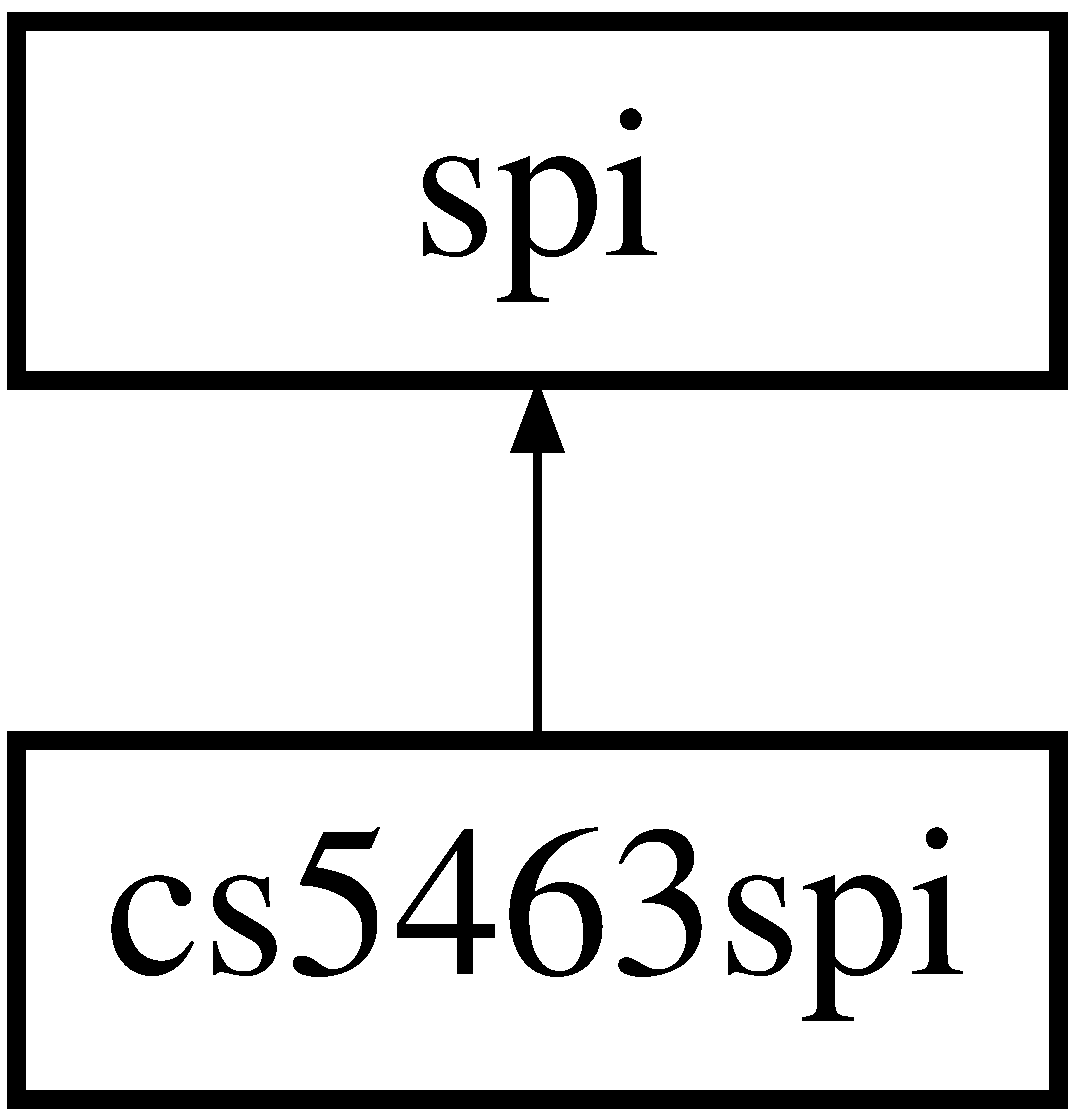
\includegraphics[height=2.000000cm]{classcs5463spi}
\end{center}
\end{figure}
\subsection*{Public Member Functions}
\begin{DoxyCompactItemize}
\item 
\hyperlink{classcs5463spi_a8b67189087e7c275a4da52992bc20324}{cs5463spi} ()
\item 
void \hyperlink{classcs5463spi_a2f1ec8b010596b4af7f64c486cdaf179}{Run} ()
\item 
bool \hyperlink{classcs5463spi_ad7baacfc87b389db65a26bd9886c6cc2}{Calibrate} (int cal\-Type=0)
\end{DoxyCompactItemize}
\subsection*{Protected Member Functions}
\begin{DoxyCompactItemize}
\item 
void \hyperlink{classcs5463spi_a8f0e36eb00a90919ae9a193b8afe69cb}{Serial\-Port\-Init} ()
\item 
void \hyperlink{classcs5463spi_afd9b989c60c3d8d24843862702dfcdea}{Serial\-Port\-Re\-Init} ()
\item 
void \hyperlink{classcs5463spi_ab61f5c633635597575dd756dd26391f3}{spi\-Init} ()
\end{DoxyCompactItemize}
\subsection*{Private Types}
\begin{DoxyCompactItemize}
\item 
enum \{ \\*
{\bfseries ic\-\_\-not}, 
{\bfseries fup}, 
{\bfseries lsd}, 
{\bfseries iod}, 
\\*
{\bfseries vod}, 
{\bfseries tod} =6, 
{\bfseries tup}, 
{\bfseries vsag} =10, 
\\*
{\bfseries ifault}, 
{\bfseries eor}, 
{\bfseries vror}, 
{\bfseries iror}, 
\\*
{\bfseries vor} =16, 
{\bfseries ior}, 
{\bfseries crdy} =20, 
{\bfseries drdy} =23
 \}
\item 
enum \{ {\bfseries i\-\_\-dc\-\_\-offset} = 1, 
{\bfseries v\-\_\-dc\-\_\-offset}, 
{\bfseries iv\-\_\-dc\-\_\-offset}
 \}
\end{DoxyCompactItemize}
\subsection*{Private Member Functions}
\begin{DoxyCompactItemize}
\item 
int \hyperlink{classcs5463spi_ac5ceba73424261fdf42f68448535ec75}{Write\-Register} (uint8\-\_\-t cmd, uint8\-\_\-t high\-Byte, uint8\-\_\-t mid\-Byte, uint8\-\_\-t low\-Byte)
\item 
int \hyperlink{classcs5463spi_a45c08ae60291209a0878b859872a9fbe}{Read\-Register} (uint8\-\_\-t cmd, uint8\-\_\-t $\ast$p\-Rxed)
\item 
int \hyperlink{classcs5463spi_a4eef4adeb61cdf3d818e410d4d5e37aa}{send\-Cmd} (uint8\-\_\-t cmd)
\item 
\hypertarget{classcs5463spi_a9e5ec18debabcf9ef375224cf08cecb0}{void {\bfseries set\-Page} (uint8\-\_\-t pg)}\label{classcs5463spi_a9e5ec18debabcf9ef375224cf08cecb0}

\item 
void \hyperlink{classcs5463spi_aafda987549f89a9917cec36f74e17874}{Sw\-Reset} ()
\item 
void \hyperlink{classcs5463spi_af398289d5aa2398af031696f58fbf2e5}{Power\-Down} (uint8\-\_\-t pw\-Cmd)
\item 
\hypertarget{classcs5463spi_a98b2af7f4a7ffe2e8281557a7ec91394}{void {\bfseries Sync} (uint8\-\_\-t sync\-Type)}\label{classcs5463spi_a98b2af7f4a7ffe2e8281557a7ec91394}

\item 
int \hyperlink{classcs5463spi_ab4061eb580d7951c6a0a1f57cef02359}{Start\-Convertion} (uint8\-\_\-t start\-Cmd)
\item 
bool \hyperlink{classcs5463spi_ad121321a0ce78ea58e1425f157b96074}{Interrupt\-Handler\-Init} (bool D\-R\-D\-Y)
\item 
bool \hyperlink{classcs5463spi_abffdb96164657da7d6c8f125c3b776ec}{Disable\-Interrupts} ()
\item 
\hypertarget{classcs5463spi_a61d65a32ed681d1bec2ab60a723502e9}{void {\bfseries Interrupt\-Handler} ()}\label{classcs5463spi_a61d65a32ed681d1bec2ab60a723502e9}

\item 
void \hyperlink{classcs5463spi_a3dca190be7b9d15e5f224caabf3ea356}{Check\-Status} (uint8\-\_\-t $\ast$status)
\item 
bool \hyperlink{classcs5463spi_af8e47c4b7ef0aa7f37e4ddedb6545508}{Check\-Status\-Ready} (int bit)
\item 
bool \hyperlink{classcs5463spi_a6607917b066f2e6733bc4b46c13af61c}{Ichann\-D\-Coffset\-Cal} ()
\item 
bool \hyperlink{classcs5463spi_a51236d9b55605eeba87c7f016b1bcf55}{Vchann\-D\-Coffset\-Cal} ()
\item 
bool \hyperlink{classcs5463spi_a825ab80592f6d90501c5f4d83977ded5}{Ichann\-A\-Coffset\-Cal} ()
\item 
bool \hyperlink{classcs5463spi_a6fdc28d935e69c70eb844c030e73654a}{Vchann\-A\-Coffset\-Cal} ()
\item 
void \hyperlink{classcs5463spi_a9213fc3397234424ce5c62dc5b13e634}{Make\-Readings} ()
\item 
\hypertarget{classcs5463spi_a7fbf4a5fbc7f415afcc74a265883c674}{\hyperlink{structcs5463ElectricityAttr}{cs5463\-Electricity\-Attr} {\bfseries get\-Read\-Values} ()}\label{classcs5463spi_a7fbf4a5fbc7f415afcc74a265883c674}

\item 
void \hyperlink{classcs5463spi_a166fefb7fbb67b265dffc6c9c07ef96b}{set\-Mode\-Spi} (uint8\-\_\-t wr\-Mode, uint8\-\_\-t rd\-Mode)
\item 
uint32\-\_\-t \hyperlink{classcs5463spi_aa85ec2bd59b4fc80c7dc59812e6d186e}{make32} (uint8\-\_\-t $\ast$var)
\end{DoxyCompactItemize}
\subsection*{Private Attributes}
\begin{DoxyCompactItemize}
\item 
\hypertarget{classcs5463spi_a781696b7e209c506e792ad0e20d79a2e}{\hyperlink{structRegReadCmd}{Reg\-Read\-Cmd} {\bfseries m\-\_\-reg\-Read\-Cmd}}\label{classcs5463spi_a781696b7e209c506e792ad0e20d79a2e}

\item 
\hypertarget{classcs5463spi_a61ca58fa6b0046b7fc1ce4d5db0bed4a}{\hyperlink{structRegWrCmd}{Reg\-Wr\-Cmd} {\bfseries m\-\_\-reg\-Wr\-Cmd}}\label{classcs5463spi_a61ca58fa6b0046b7fc1ce4d5db0bed4a}

\item 
\hypertarget{classcs5463spi_a1bcaa5292a33a2dc7a61ff31ba436d0c}{\hyperlink{structcs5463Commands}{cs5463\-Commands} {\bfseries m\-\_\-cmds}}\label{classcs5463spi_a1bcaa5292a33a2dc7a61ff31ba436d0c}

\item 
\hypertarget{classcs5463spi_a47886abba6bf33a5683f56ef9c5ff1cc}{\hyperlink{structcs5463ElectricityAttr}{cs5463\-Electricity\-Attr} {\bfseries m\-\_\-electricity\-Attr}}\label{classcs5463spi_a47886abba6bf33a5683f56ef9c5ff1cc}

\item 
\hypertarget{classcs5463spi_aec97d1e881b52d65cb85b20def733527}{\hyperlink{structcs5463spiParams}{cs5463spi\-Params} {\bfseries m\-\_\-spi\-Params}}\label{classcs5463spi_aec97d1e881b52d65cb85b20def733527}

\item 
\hypertarget{classcs5463spi_af02787a5e4858c19b44215b5b955efa5}{\hyperlink{structcs5463sysCalOffsetVals}{cs5463sys\-Cal\-Offset\-Vals} {\bfseries m\-\_\-sys\-Cal\-Offset}}\label{classcs5463spi_af02787a5e4858c19b44215b5b955efa5}

\item 
\hypertarget{classcs5463spi_a26e1ce56ca06dba3d73c63c8b10a4214}{\hyperlink{structcs5463sysCalGainVals}{cs5463sys\-Cal\-Gain\-Vals} {\bfseries m\-\_\-sys\-Cal\-Gain}}\label{classcs5463spi_a26e1ce56ca06dba3d73c63c8b10a4214}

\item 
\hypertarget{classcs5463spi_a4a13325c4a439e50ebf0276048cf542e}{std\-::vector$<$ std\-::string $>$ {\bfseries m\-\_\-status\-Warn}}\label{classcs5463spi_a4a13325c4a439e50ebf0276048cf542e}

\end{DoxyCompactItemize}
\subsection*{Additional Inherited Members}


\subsection{Detailed Description}
Calibration Fudge Factors Class that defines the functionalities of C\-S5463. It derives from the spi class 

\subsection{Constructor \& Destructor Documentation}
\hypertarget{classcs5463spi_a8b67189087e7c275a4da52992bc20324}{\index{cs5463spi@{cs5463spi}!cs5463spi@{cs5463spi}}
\index{cs5463spi@{cs5463spi}!cs5463spi@{cs5463spi}}
\subsubsection[{cs5463spi}]{\setlength{\rightskip}{0pt plus 5cm}cs5463spi\-::cs5463spi (
\begin{DoxyParamCaption}
{}
\end{DoxyParamCaption}
)}}\label{classcs5463spi_a8b67189087e7c275a4da52992bc20324}
Constructor 

\subsection{Member Function Documentation}
\hypertarget{classcs5463spi_ad7baacfc87b389db65a26bd9886c6cc2}{\index{cs5463spi@{cs5463spi}!Calibrate@{Calibrate}}
\index{Calibrate@{Calibrate}!cs5463spi@{cs5463spi}}
\subsubsection[{Calibrate}]{\setlength{\rightskip}{0pt plus 5cm}bool cs5463spi\-::\-Calibrate (
\begin{DoxyParamCaption}
\item[{int}]{cal\-Type = {\ttfamily 0}}
\end{DoxyParamCaption}
)\hspace{0.3cm}{\ttfamily [virtual]}}}\label{classcs5463spi_ad7baacfc87b389db65a26bd9886c6cc2}
Calibrate Method, public domain 

Reimplemented from \hyperlink{classspi}{spi}.

\hypertarget{classcs5463spi_a3dca190be7b9d15e5f224caabf3ea356}{\index{cs5463spi@{cs5463spi}!Check\-Status@{Check\-Status}}
\index{Check\-Status@{Check\-Status}!cs5463spi@{cs5463spi}}
\subsubsection[{Check\-Status}]{\setlength{\rightskip}{0pt plus 5cm}void cs5463spi\-::\-Check\-Status (
\begin{DoxyParamCaption}
\item[{uint8\-\_\-t $\ast$}]{status}
\end{DoxyParamCaption}
)\hspace{0.3cm}{\ttfamily [private]}}}\label{classcs5463spi_a3dca190be7b9d15e5f224caabf3ea356}
Check\-Status \hypertarget{classcs5463spi_af8e47c4b7ef0aa7f37e4ddedb6545508}{\index{cs5463spi@{cs5463spi}!Check\-Status\-Ready@{Check\-Status\-Ready}}
\index{Check\-Status\-Ready@{Check\-Status\-Ready}!cs5463spi@{cs5463spi}}
\subsubsection[{Check\-Status\-Ready}]{\setlength{\rightskip}{0pt plus 5cm}bool cs5463spi\-::\-Check\-Status\-Ready (
\begin{DoxyParamCaption}
\item[{int}]{bit}
\end{DoxyParamCaption}
)\hspace{0.3cm}{\ttfamily [private]}}}\label{classcs5463spi_af8e47c4b7ef0aa7f37e4ddedb6545508}
bool Check\-Status\-Ready(uint8\-\_\-t$\ast$ byte, int bit); check data ready and convertion ready \hypertarget{classcs5463spi_abffdb96164657da7d6c8f125c3b776ec}{\index{cs5463spi@{cs5463spi}!Disable\-Interrupts@{Disable\-Interrupts}}
\index{Disable\-Interrupts@{Disable\-Interrupts}!cs5463spi@{cs5463spi}}
\subsubsection[{Disable\-Interrupts}]{\setlength{\rightskip}{0pt plus 5cm}bool cs5463spi\-::\-Disable\-Interrupts (
\begin{DoxyParamCaption}
{}
\end{DoxyParamCaption}
)\hspace{0.3cm}{\ttfamily [private]}}}\label{classcs5463spi_abffdb96164657da7d6c8f125c3b776ec}
\hyperlink{classcs5463spi_abffdb96164657da7d6c8f125c3b776ec}{Disable\-Interrupts()} \hypertarget{classcs5463spi_a825ab80592f6d90501c5f4d83977ded5}{\index{cs5463spi@{cs5463spi}!Ichann\-A\-Coffset\-Cal@{Ichann\-A\-Coffset\-Cal}}
\index{Ichann\-A\-Coffset\-Cal@{Ichann\-A\-Coffset\-Cal}!cs5463spi@{cs5463spi}}
\subsubsection[{Ichann\-A\-Coffset\-Cal}]{\setlength{\rightskip}{0pt plus 5cm}bool cs5463spi\-::\-Ichann\-A\-Coffset\-Cal (
\begin{DoxyParamCaption}
{}
\end{DoxyParamCaption}
)\hspace{0.3cm}{\ttfamily [private]}}}\label{classcs5463spi_a825ab80592f6d90501c5f4d83977ded5}
Performs I Channel A\-C Offset Calibration \hypertarget{classcs5463spi_a6607917b066f2e6733bc4b46c13af61c}{\index{cs5463spi@{cs5463spi}!Ichann\-D\-Coffset\-Cal@{Ichann\-D\-Coffset\-Cal}}
\index{Ichann\-D\-Coffset\-Cal@{Ichann\-D\-Coffset\-Cal}!cs5463spi@{cs5463spi}}
\subsubsection[{Ichann\-D\-Coffset\-Cal}]{\setlength{\rightskip}{0pt plus 5cm}bool cs5463spi\-::\-Ichann\-D\-Coffset\-Cal (
\begin{DoxyParamCaption}
{}
\end{DoxyParamCaption}
)\hspace{0.3cm}{\ttfamily [private]}}}\label{classcs5463spi_a6607917b066f2e6733bc4b46c13af61c}
Performs I Channel D\-C Offset Calibration \hypertarget{classcs5463spi_ad121321a0ce78ea58e1425f157b96074}{\index{cs5463spi@{cs5463spi}!Interrupt\-Handler\-Init@{Interrupt\-Handler\-Init}}
\index{Interrupt\-Handler\-Init@{Interrupt\-Handler\-Init}!cs5463spi@{cs5463spi}}
\subsubsection[{Interrupt\-Handler\-Init}]{\setlength{\rightskip}{0pt plus 5cm}bool cs5463spi\-::\-Interrupt\-Handler\-Init (
\begin{DoxyParamCaption}
\item[{bool}]{D\-R\-D\-Y}
\end{DoxyParamCaption}
)\hspace{0.3cm}{\ttfamily [private]}}}\label{classcs5463spi_ad121321a0ce78ea58e1425f157b96074}
Enables Interrupts \hypertarget{classcs5463spi_aa85ec2bd59b4fc80c7dc59812e6d186e}{\index{cs5463spi@{cs5463spi}!make32@{make32}}
\index{make32@{make32}!cs5463spi@{cs5463spi}}
\subsubsection[{make32}]{\setlength{\rightskip}{0pt plus 5cm}uint32\-\_\-t cs5463spi\-::make32 (
\begin{DoxyParamCaption}
\item[{uint8\-\_\-t $\ast$}]{var}
\end{DoxyParamCaption}
)\hspace{0.3cm}{\ttfamily [private]}}}\label{classcs5463spi_aa85ec2bd59b4fc80c7dc59812e6d186e}
Makes 3 bytes into a 32 bit number; \hypertarget{classcs5463spi_a9213fc3397234424ce5c62dc5b13e634}{\index{cs5463spi@{cs5463spi}!Make\-Readings@{Make\-Readings}}
\index{Make\-Readings@{Make\-Readings}!cs5463spi@{cs5463spi}}
\subsubsection[{Make\-Readings}]{\setlength{\rightskip}{0pt plus 5cm}void cs5463spi\-::\-Make\-Readings (
\begin{DoxyParamCaption}
{}
\end{DoxyParamCaption}
)\hspace{0.3cm}{\ttfamily [private]}}}\label{classcs5463spi_a9213fc3397234424ce5c62dc5b13e634}
Starts register reading. This is an overridden function. \hypertarget{classcs5463spi_af398289d5aa2398af031696f58fbf2e5}{\index{cs5463spi@{cs5463spi}!Power\-Down@{Power\-Down}}
\index{Power\-Down@{Power\-Down}!cs5463spi@{cs5463spi}}
\subsubsection[{Power\-Down}]{\setlength{\rightskip}{0pt plus 5cm}void cs5463spi\-::\-Power\-Down (
\begin{DoxyParamCaption}
\item[{uint8\-\_\-t}]{pw\-Cmd}
\end{DoxyParamCaption}
)\hspace{0.3cm}{\ttfamily [private]}}}\label{classcs5463spi_af398289d5aa2398af031696f58fbf2e5}
Power Down \hypertarget{classcs5463spi_a45c08ae60291209a0878b859872a9fbe}{\index{cs5463spi@{cs5463spi}!Read\-Register@{Read\-Register}}
\index{Read\-Register@{Read\-Register}!cs5463spi@{cs5463spi}}
\subsubsection[{Read\-Register}]{\setlength{\rightskip}{0pt plus 5cm}int cs5463spi\-::\-Read\-Register (
\begin{DoxyParamCaption}
\item[{uint8\-\_\-t}]{cmd, }
\item[{uint8\-\_\-t $\ast$}]{p\-Rxed}
\end{DoxyParamCaption}
)\hspace{0.3cm}{\ttfamily [private]}}}\label{classcs5463spi_a45c08ae60291209a0878b859872a9fbe}
Reads register value. This is a overridden function. Spi mode 1 is used to read data. (data is read on the clock falling edge. \hypertarget{classcs5463spi_a2f1ec8b010596b4af7f64c486cdaf179}{\index{cs5463spi@{cs5463spi}!Run@{Run}}
\index{Run@{Run}!cs5463spi@{cs5463spi}}
\subsubsection[{Run}]{\setlength{\rightskip}{0pt plus 5cm}void cs5463spi\-::\-Run (
\begin{DoxyParamCaption}
{}
\end{DoxyParamCaption}
)\hspace{0.3cm}{\ttfamily [virtual]}}}\label{classcs5463spi_a2f1ec8b010596b4af7f64c486cdaf179}
Reads all required Electrical parameters 

Reimplemented from \hyperlink{classspi}{spi}.

\hypertarget{classcs5463spi_a4eef4adeb61cdf3d818e410d4d5e37aa}{\index{cs5463spi@{cs5463spi}!send\-Cmd@{send\-Cmd}}
\index{send\-Cmd@{send\-Cmd}!cs5463spi@{cs5463spi}}
\subsubsection[{send\-Cmd}]{\setlength{\rightskip}{0pt plus 5cm}int cs5463spi\-::send\-Cmd (
\begin{DoxyParamCaption}
\item[{uint8\-\_\-t}]{cmd}
\end{DoxyParamCaption}
)\hspace{0.3cm}{\ttfamily [private]}}}\label{classcs5463spi_a4eef4adeb61cdf3d818e410d4d5e37aa}
Sets command to register Commands are 8 bit in length (one byte) \hypertarget{classcs5463spi_a8f0e36eb00a90919ae9a193b8afe69cb}{\index{cs5463spi@{cs5463spi}!Serial\-Port\-Init@{Serial\-Port\-Init}}
\index{Serial\-Port\-Init@{Serial\-Port\-Init}!cs5463spi@{cs5463spi}}
\subsubsection[{Serial\-Port\-Init}]{\setlength{\rightskip}{0pt plus 5cm}void cs5463spi\-::\-Serial\-Port\-Init (
\begin{DoxyParamCaption}
{}
\end{DoxyParamCaption}
)\hspace{0.3cm}{\ttfamily [protected]}, {\ttfamily [virtual]}}}\label{classcs5463spi_a8f0e36eb00a90919ae9a193b8afe69cb}
Initializes the C\-S5463's S\-P\-I. This is an overridden function. 

Reimplemented from \hyperlink{classspi}{spi}.

\hypertarget{classcs5463spi_afd9b989c60c3d8d24843862702dfcdea}{\index{cs5463spi@{cs5463spi}!Serial\-Port\-Re\-Init@{Serial\-Port\-Re\-Init}}
\index{Serial\-Port\-Re\-Init@{Serial\-Port\-Re\-Init}!cs5463spi@{cs5463spi}}
\subsubsection[{Serial\-Port\-Re\-Init}]{\setlength{\rightskip}{0pt plus 5cm}void cs5463spi\-::\-Serial\-Port\-Re\-Init (
\begin{DoxyParamCaption}
{}
\end{DoxyParamCaption}
)\hspace{0.3cm}{\ttfamily [protected]}}}\label{classcs5463spi_afd9b989c60c3d8d24843862702dfcdea}
This function reinitializes the C\-S5463 serial port \hypertarget{classcs5463spi_a166fefb7fbb67b265dffc6c9c07ef96b}{\index{cs5463spi@{cs5463spi}!set\-Mode\-Spi@{set\-Mode\-Spi}}
\index{set\-Mode\-Spi@{set\-Mode\-Spi}!cs5463spi@{cs5463spi}}
\subsubsection[{set\-Mode\-Spi}]{\setlength{\rightskip}{0pt plus 5cm}void cs5463spi\-::set\-Mode\-Spi (
\begin{DoxyParamCaption}
\item[{uint8\-\_\-t}]{wr\-Mode, }
\item[{uint8\-\_\-t}]{rd\-Mode}
\end{DoxyParamCaption}
)\hspace{0.3cm}{\ttfamily [private]}}}\label{classcs5463spi_a166fefb7fbb67b265dffc6c9c07ef96b}
Sets the S\-P\-I mode. This is needed as the C\-S5463 has different spi modes for data reads and data writes. \hypertarget{classcs5463spi_ab61f5c633635597575dd756dd26391f3}{\index{cs5463spi@{cs5463spi}!spi\-Init@{spi\-Init}}
\index{spi\-Init@{spi\-Init}!cs5463spi@{cs5463spi}}
\subsubsection[{spi\-Init}]{\setlength{\rightskip}{0pt plus 5cm}void cs5463spi\-::spi\-Init (
\begin{DoxyParamCaption}
{}
\end{DoxyParamCaption}
)\hspace{0.3cm}{\ttfamily [protected]}, {\ttfamily [virtual]}}}\label{classcs5463spi_ab61f5c633635597575dd756dd26391f3}
Initilalizes spi Device. 

Reimplemented from \hyperlink{classspi_af6b5a441ef9014df209fa3803d0fa68f}{spi}.

\hypertarget{classcs5463spi_ab4061eb580d7951c6a0a1f57cef02359}{\index{cs5463spi@{cs5463spi}!Start\-Convertion@{Start\-Convertion}}
\index{Start\-Convertion@{Start\-Convertion}!cs5463spi@{cs5463spi}}
\subsubsection[{Start\-Convertion}]{\setlength{\rightskip}{0pt plus 5cm}int cs5463spi\-::\-Start\-Convertion (
\begin{DoxyParamCaption}
\item[{uint8\-\_\-t}]{start\-Cmd}
\end{DoxyParamCaption}
)\hspace{0.3cm}{\ttfamily [private]}}}\label{classcs5463spi_ab4061eb580d7951c6a0a1f57cef02359}
Starts C\-S5463 convertion. \hypertarget{classcs5463spi_aafda987549f89a9917cec36f74e17874}{\index{cs5463spi@{cs5463spi}!Sw\-Reset@{Sw\-Reset}}
\index{Sw\-Reset@{Sw\-Reset}!cs5463spi@{cs5463spi}}
\subsubsection[{Sw\-Reset}]{\setlength{\rightskip}{0pt plus 5cm}void cs5463spi\-::\-Sw\-Reset (
\begin{DoxyParamCaption}
{}
\end{DoxyParamCaption}
)\hspace{0.3cm}{\ttfamily [private]}}}\label{classcs5463spi_aafda987549f89a9917cec36f74e17874}
Performs a software reset of C\-S5463 S\-P\-I \hypertarget{classcs5463spi_a6fdc28d935e69c70eb844c030e73654a}{\index{cs5463spi@{cs5463spi}!Vchann\-A\-Coffset\-Cal@{Vchann\-A\-Coffset\-Cal}}
\index{Vchann\-A\-Coffset\-Cal@{Vchann\-A\-Coffset\-Cal}!cs5463spi@{cs5463spi}}
\subsubsection[{Vchann\-A\-Coffset\-Cal}]{\setlength{\rightskip}{0pt plus 5cm}bool cs5463spi\-::\-Vchann\-A\-Coffset\-Cal (
\begin{DoxyParamCaption}
{}
\end{DoxyParamCaption}
)\hspace{0.3cm}{\ttfamily [private]}}}\label{classcs5463spi_a6fdc28d935e69c70eb844c030e73654a}
Performs V Channel A\-C Offset Calibration \hypertarget{classcs5463spi_a51236d9b55605eeba87c7f016b1bcf55}{\index{cs5463spi@{cs5463spi}!Vchann\-D\-Coffset\-Cal@{Vchann\-D\-Coffset\-Cal}}
\index{Vchann\-D\-Coffset\-Cal@{Vchann\-D\-Coffset\-Cal}!cs5463spi@{cs5463spi}}
\subsubsection[{Vchann\-D\-Coffset\-Cal}]{\setlength{\rightskip}{0pt plus 5cm}bool cs5463spi\-::\-Vchann\-D\-Coffset\-Cal (
\begin{DoxyParamCaption}
{}
\end{DoxyParamCaption}
)\hspace{0.3cm}{\ttfamily [private]}}}\label{classcs5463spi_a51236d9b55605eeba87c7f016b1bcf55}
Performs V Channel D\-C Offset calibration \hypertarget{classcs5463spi_ac5ceba73424261fdf42f68448535ec75}{\index{cs5463spi@{cs5463spi}!Write\-Register@{Write\-Register}}
\index{Write\-Register@{Write\-Register}!cs5463spi@{cs5463spi}}
\subsubsection[{Write\-Register}]{\setlength{\rightskip}{0pt plus 5cm}int cs5463spi\-::\-Write\-Register (
\begin{DoxyParamCaption}
\item[{uint8\-\_\-t}]{cmd, }
\item[{uint8\-\_\-t}]{high\-Byte, }
\item[{uint8\-\_\-t}]{mid\-Byte, }
\item[{uint8\-\_\-t}]{low\-Byte}
\end{DoxyParamCaption}
)\hspace{0.3cm}{\ttfamily [private]}}}\label{classcs5463spi_ac5ceba73424261fdf42f68448535ec75}
Writes command/value to register 

The documentation for this class was generated from the following files\-:\begin{DoxyCompactItemize}
\item 
cs5463\-\_\-spi.\-h\item 
cs5463\-\_\-spi.\-cpp\end{DoxyCompactItemize}

\hypertarget{structcs5463spiParams}{\section{cs5463spi\-Params Struct Reference}
\label{structcs5463spiParams}\index{cs5463spi\-Params@{cs5463spi\-Params}}
}


{\ttfamily \#include $<$cs5463\-\_\-spi.\-h$>$}

\subsection*{Static Public Attributes}
\begin{DoxyCompactItemize}
\item 
\hypertarget{structcs5463spiParams_ae2777803bb5b41ebe0a0d758d28f4ded}{static const uint8\-\_\-t {\bfseries B\-I\-T\-\_\-\-O\-R\-D\-E\-R} = 0}\label{structcs5463spiParams_ae2777803bb5b41ebe0a0d758d28f4ded}

\item 
\hypertarget{structcs5463spiParams_a4cd49ecac3420ed8a8e885f2868cb093}{static const uint8\-\_\-t {\bfseries M\-O\-D\-E\-\_\-0} = 0}\label{structcs5463spiParams_a4cd49ecac3420ed8a8e885f2868cb093}

\item 
\hypertarget{structcs5463spiParams_a4d76eb638a9dd8ec0162fd6ccde5e81d}{static const uint8\-\_\-t {\bfseries M\-O\-D\-E\-\_\-1} = 1}\label{structcs5463spiParams_a4d76eb638a9dd8ec0162fd6ccde5e81d}

\item 
\hypertarget{structcs5463spiParams_a381cde3229b78cf9502d44912898423b}{static const uint8\-\_\-t {\bfseries B\-P\-W} = 8}\label{structcs5463spiParams_a381cde3229b78cf9502d44912898423b}

\item 
\hypertarget{structcs5463spiParams_a63fd68edbc4069935ba250a29cc37f8d}{static const uint32\-\_\-t {\bfseries M\-A\-X\-\_\-\-F\-R\-E\-Q} = 2000000}\label{structcs5463spiParams_a63fd68edbc4069935ba250a29cc37f8d}

\end{DoxyCompactItemize}


\subsection{Detailed Description}
C\-S5463 local spi parameters. 

The documentation for this struct was generated from the following file\-:\begin{DoxyCompactItemize}
\item 
cs5463\-\_\-spi.\-h\end{DoxyCompactItemize}

\hypertarget{structcs5463sysCalGainVals}{\section{cs5463sys\-Cal\-Gain\-Vals Struct Reference}
\label{structcs5463sysCalGainVals}\index{cs5463sys\-Cal\-Gain\-Vals@{cs5463sys\-Cal\-Gain\-Vals}}
}
\subsection*{Static Public Attributes}
\begin{DoxyCompactItemize}
\item 
\hypertarget{structcs5463sysCalGainVals_aa3cd084b170af11b56082bb0cd05d46d}{static const uint8\-\_\-t {\bfseries I\-\_\-\-C\-H\-A\-N\-\_\-\-D\-C\-\_\-\-G\-A\-I\-N} = 0x\-C\-A}\label{structcs5463sysCalGainVals_aa3cd084b170af11b56082bb0cd05d46d}

\item 
\hypertarget{structcs5463sysCalGainVals_ae30afd0d60a3e489c179dd8e4e94cb34}{static const uint8\-\_\-t {\bfseries V\-\_\-\-C\-H\-A\-N\-\_\-\-D\-C\-\_\-\-G\-A\-I\-N} = 0x\-D2}\label{structcs5463sysCalGainVals_ae30afd0d60a3e489c179dd8e4e94cb34}

\item 
\hypertarget{structcs5463sysCalGainVals_a79e875dc5137298a2ea06e9199fea354}{static const uint8\-\_\-t {\bfseries I\-\_\-\-A\-N\-D\-\_\-\-V\-\_\-\-D\-C\-\_\-\-G\-A\-I\-N} = 0x\-D\-A}\label{structcs5463sysCalGainVals_a79e875dc5137298a2ea06e9199fea354}

\item 
\hypertarget{structcs5463sysCalGainVals_aefe1ae2f262bd5e323d29774e7f023ba}{static const uint8\-\_\-t {\bfseries I\-\_\-\-C\-H\-A\-N\-\_\-\-A\-C\-\_\-\-G\-A\-I\-N} = 0x\-C3}\label{structcs5463sysCalGainVals_aefe1ae2f262bd5e323d29774e7f023ba}

\item 
\hypertarget{structcs5463sysCalGainVals_a517bbf6253232087ff21d55ddae7045f}{static const uint8\-\_\-t {\bfseries V\-\_\-\-C\-H\-A\-N\-\_\-\-A\-C\-\_\-\-G\-A\-I\-N} = 0x\-D6}\label{structcs5463sysCalGainVals_a517bbf6253232087ff21d55ddae7045f}

\item 
\hypertarget{structcs5463sysCalGainVals_aa27c74c8c8affbdd1a786cbee5aaf48c}{static const uint8\-\_\-t {\bfseries I\-\_\-\-A\-N\-D\-\_\-\-V\-\_\-\-A\-C\-\_\-\-G\-A\-I\-N} = 0x\-D\-E}\label{structcs5463sysCalGainVals_aa27c74c8c8affbdd1a786cbee5aaf48c}

\end{DoxyCompactItemize}


The documentation for this struct was generated from the following file\-:\begin{DoxyCompactItemize}
\item 
cs5463\-\_\-spi.\-h\end{DoxyCompactItemize}

\hypertarget{structcs5463sysCalOffsetVals}{\section{cs5463sys\-Cal\-Offset\-Vals Struct Reference}
\label{structcs5463sysCalOffsetVals}\index{cs5463sys\-Cal\-Offset\-Vals@{cs5463sys\-Cal\-Offset\-Vals}}
}


{\ttfamily \#include $<$cs5463\-\_\-spi.\-h$>$}

\subsection*{Static Public Attributes}
\begin{DoxyCompactItemize}
\item 
\hypertarget{structcs5463sysCalOffsetVals_a1e44d7257eb422962ef39df73847b2ae}{static const uint8\-\_\-t {\bfseries I\-\_\-\-C\-H\-A\-N\-\_\-\-D\-C\-\_\-\-O\-F\-F\-S\-E\-T} = 0x\-C9}\label{structcs5463sysCalOffsetVals_a1e44d7257eb422962ef39df73847b2ae}

\item 
\hypertarget{structcs5463sysCalOffsetVals_a8efca918c7cfd211922dd61ab614809c}{static const uint8\-\_\-t {\bfseries V\-\_\-\-C\-H\-A\-N\-\_\-\-D\-C\-\_\-\-O\-F\-F\-S\-E\-T} = 0x\-D1}\label{structcs5463sysCalOffsetVals_a8efca918c7cfd211922dd61ab614809c}

\item 
\hypertarget{structcs5463sysCalOffsetVals_a16004ae7e2193b0e755eb1a3ecd220d3}{static const uint8\-\_\-t {\bfseries I\-\_\-\-A\-N\-D\-\_\-\-V\-\_\-\-D\-C\-\_\-\-O\-F\-F\-S\-E\-T} = 0x\-D9}\label{structcs5463sysCalOffsetVals_a16004ae7e2193b0e755eb1a3ecd220d3}

\item 
\hypertarget{structcs5463sysCalOffsetVals_adaad0c0f33d010b87241ac380b9c3543}{static const uint8\-\_\-t {\bfseries I\-\_\-\-C\-H\-A\-N\-\_\-\-A\-C\-\_\-\-O\-F\-F\-S\-E\-T} = 0x\-C\-D}\label{structcs5463sysCalOffsetVals_adaad0c0f33d010b87241ac380b9c3543}

\item 
\hypertarget{structcs5463sysCalOffsetVals_a0df94d3f197208610a2bb9e63f9100ee}{static const uint8\-\_\-t {\bfseries V\-\_\-\-C\-H\-A\-N\-\_\-\-A\-C\-\_\-\-O\-F\-F\-S\-E\-T} = 0x\-D5}\label{structcs5463sysCalOffsetVals_a0df94d3f197208610a2bb9e63f9100ee}

\item 
\hypertarget{structcs5463sysCalOffsetVals_a912d3d1f76e999f1632ea6a72d1af5ad}{static const uint8\-\_\-t {\bfseries I\-\_\-\-A\-N\-D\-\_\-\-V\-\_\-\-A\-C\-\_\-\-O\-F\-F\-S\-E\-T} = 0x\-D\-D}\label{structcs5463sysCalOffsetVals_a912d3d1f76e999f1632ea6a72d1af5ad}

\end{DoxyCompactItemize}


\subsection{Detailed Description}
C\-S5463 Commands\-: System Calibrations 

The documentation for this struct was generated from the following file\-:\begin{DoxyCompactItemize}
\item 
cs5463\-\_\-spi.\-h\end{DoxyCompactItemize}

\hypertarget{classLogger}{\section{Logger Class Reference}
\label{classLogger}\index{Logger@{Logger}}
}
\subsection*{Public Types}
\begin{DoxyCompactItemize}
\item 
enum {\bfseries Priority} \{ \\*
{\bfseries D\-E\-B\-U\-G}, 
{\bfseries C\-O\-N\-F\-I\-G}, 
{\bfseries I\-N\-F\-O}, 
{\bfseries W\-A\-R\-N\-I\-N\-G}, 
\\*
{\bfseries E\-R\-R\-O\-R}
 \}
\end{DoxyCompactItemize}
\subsection*{Public Member Functions}
\begin{DoxyCompactItemize}
\item 
\hypertarget{classLogger_ad766b6ac85f82411a6f25af21eea58d7}{void {\bfseries Write\-Read\-Remote} (const string \&message)}\label{classLogger_ad766b6ac85f82411a6f25af21eea58d7}

\item 
\hypertarget{classLogger_a16da1083e70f46051275d4ac208c3626}{void {\bfseries Write\-Local} (int facility, int priority, const string \&message)}\label{classLogger_a16da1083e70f46051275d4ac208c3626}

\end{DoxyCompactItemize}
\subsection*{Static Public Member Functions}
\begin{DoxyCompactItemize}
\item 
\hypertarget{classLogger_aa35f17d5b79217f4b5c43dcb44b97746}{static \hyperlink{classLogger}{Logger} $\ast$ {\bfseries Instance} (const string \&log\-File, \hyperlink{classClientSocket}{Client\-Socket} $\ast$p\-Socket\-Handler, \hyperlink{structloggerInfo}{logger\-Info} $\ast$p\-My\-Logger\-Info)}\label{classLogger_aa35f17d5b79217f4b5c43dcb44b97746}

\item 
\hypertarget{classLogger_a45f0936b9f16c4f8f93ca409a9486e94}{static void {\bfseries Stop\-Instance} ()}\label{classLogger_a45f0936b9f16c4f8f93ca409a9486e94}

\end{DoxyCompactItemize}
\subsection*{Private Member Functions}
\begin{DoxyCompactItemize}
\item 
\hypertarget{classLogger_a2c5d5039e76ef20903ce7cfbc8030d47}{{\bfseries Logger} (const \hyperlink{classLogger}{Logger} \&logger)}\label{classLogger_a2c5d5039e76ef20903ce7cfbc8030d47}

\item 
\hypertarget{classLogger_a400dd030dcec25d075f87202e880c5b9}{\hyperlink{classLogger}{Logger} \& {\bfseries operator=} (const \hyperlink{classLogger}{Logger} \&logger)}\label{classLogger_a400dd030dcec25d075f87202e880c5b9}

\end{DoxyCompactItemize}
\subsection*{Private Attributes}
\begin{DoxyCompactItemize}
\item 
\hypertarget{classLogger_a79d231b8f8c27d0c0b6f963f753b2be1}{bool {\bfseries active}}\label{classLogger_a79d231b8f8c27d0c0b6f963f753b2be1}

\item 
\hypertarget{classLogger_afea7dca3fd4d8f909bb5d5906d2b5293}{ofstream {\bfseries file\-Stream}}\label{classLogger_afea7dca3fd4d8f909bb5d5906d2b5293}

\item 
\hypertarget{classLogger_a2d408b566a4a54aafb391ca9ed3ffa03}{Priority {\bfseries min\-Priority}}\label{classLogger_a2d408b566a4a54aafb391ca9ed3ffa03}

\item 
\hypertarget{classLogger_a1a3d4ce692f3d78cc4f62dec79cb1685}{\hyperlink{classClientSocket}{Client\-Socket} $\ast$ {\bfseries p\-Socket\-Handler}}\label{classLogger_a1a3d4ce692f3d78cc4f62dec79cb1685}

\item 
\hypertarget{classLogger_a4a6cbed1d68b500ccd2bf6f8af486e88}{\hyperlink{structloggerInfo}{logger\-Info} $\ast$ {\bfseries p\-Logger\-Info}}\label{classLogger_a4a6cbed1d68b500ccd2bf6f8af486e88}

\end{DoxyCompactItemize}
\subsection*{Static Private Attributes}
\begin{DoxyCompactItemize}
\item 
\hypertarget{classLogger_af34a222ad5ec1399d6c529e0c4001b36}{static const string {\bfseries P\-R\-I\-O\-R\-I\-T\-Y\-\_\-\-N\-A\-M\-E\-S} \mbox{[}$\,$\mbox{]}}\label{classLogger_af34a222ad5ec1399d6c529e0c4001b36}

\item 
\hypertarget{classLogger_a5e9fd267cd621afeb1201131071425ea}{static \hyperlink{classLogger}{Logger} $\ast$ {\bfseries instance} = N\-U\-L\-L}\label{classLogger_a5e9fd267cd621afeb1201131071425ea}

\end{DoxyCompactItemize}


The documentation for this class was generated from the following files\-:\begin{DoxyCompactItemize}
\item 
common/Logger.\-h\item 
common/Logger.\-cpp\end{DoxyCompactItemize}

\hypertarget{structloggerInfo}{\section{logger\-Info Struct Reference}
\label{structloggerInfo}\index{logger\-Info@{logger\-Info}}
}
\subsection*{Data Fields}
\begin{DoxyCompactItemize}
\item 
\hypertarget{structloggerInfo_addba2d28a1df00c5e04dcee47434cf09}{std\-::string {\bfseries client\-Name}}\label{structloggerInfo_addba2d28a1df00c5e04dcee47434cf09}

\item 
\hypertarget{structloggerInfo_afa1407f38913794ea9933c15e8684e60}{std\-::string {\bfseries app\-Name}}\label{structloggerInfo_afa1407f38913794ea9933c15e8684e60}

\item 
\hypertarget{structloggerInfo_a383138c846b52e02bce1767698e22fc8}{std\-::string {\bfseries pid\-No}}\label{structloggerInfo_a383138c846b52e02bce1767698e22fc8}

\end{DoxyCompactItemize}


The documentation for this struct was generated from the following file\-:\begin{DoxyCompactItemize}
\item 
common/Logger.\-h\end{DoxyCompactItemize}

\hypertarget{structRegReadCmd}{\section{Reg\-Read\-Cmd Struct Reference}
\label{structRegReadCmd}\index{Reg\-Read\-Cmd@{Reg\-Read\-Cmd}}
}


{\ttfamily \#include $<$cs5463\-\_\-spi.\-h$>$}

\subsection*{Static Public Attributes}
\begin{DoxyCompactItemize}
\item 
\hypertarget{structRegReadCmd_adb8d43d2f043bc11f9c573fb132d4a0f}{static const uint8\-\_\-t {\bfseries C\-O\-N\-F} = 0x00}\label{structRegReadCmd_adb8d43d2f043bc11f9c573fb132d4a0f}

\item 
\hypertarget{structRegReadCmd_ab22a2918bdd7f4dc27d1c6347b889e7b}{static const uint8\-\_\-t {\bfseries I\-\_\-\-D\-C\-\_\-\-O\-F\-F} = 0x02}\label{structRegReadCmd_ab22a2918bdd7f4dc27d1c6347b889e7b}

\item 
\hypertarget{structRegReadCmd_ad17e24efa81e98ec9f2fcd631ca91dfe}{static const uint8\-\_\-t {\bfseries I\-\_\-\-G\-A\-I\-N} = 0x04}\label{structRegReadCmd_ad17e24efa81e98ec9f2fcd631ca91dfe}

\item 
\hypertarget{structRegReadCmd_acb4395b2cee4dd5db2c8ab84368c5f69}{static const uint8\-\_\-t {\bfseries V\-\_\-\-D\-C\-\_\-\-O\-F\-F} = 0x06}\label{structRegReadCmd_acb4395b2cee4dd5db2c8ab84368c5f69}

\item 
\hypertarget{structRegReadCmd_ae6fb80bf7aec0bc7f3dba25fb2429dda}{static const uint8\-\_\-t {\bfseries V\-\_\-\-G\-A\-I\-N} = 0x08}\label{structRegReadCmd_ae6fb80bf7aec0bc7f3dba25fb2429dda}

\item 
\hypertarget{structRegReadCmd_aee7bc23bec4480bb1638cf2af169a302}{static const uint8\-\_\-t {\bfseries C\-Y\-C\-L\-E\-\_\-\-C\-N\-T} = 0x0\-A}\label{structRegReadCmd_aee7bc23bec4480bb1638cf2af169a302}

\item 
\hypertarget{structRegReadCmd_aac0af782ab00eada9bbd95e1e58cde28}{static const uint8\-\_\-t {\bfseries P\-U\-L\-S\-E\-\_\-\-R\-A\-T\-E} = 0x0\-C}\label{structRegReadCmd_aac0af782ab00eada9bbd95e1e58cde28}

\item 
\hypertarget{structRegReadCmd_a6a60bf40d92eb138d8ad908e81eb7167}{static const uint8\-\_\-t {\bfseries I\-\_\-\-I\-N\-S} = 0x0\-E}\label{structRegReadCmd_a6a60bf40d92eb138d8ad908e81eb7167}

\item 
\hypertarget{structRegReadCmd_a6504ad862aac69a6d016388d9710cbe3}{static const uint8\-\_\-t {\bfseries V\-\_\-\-I\-N\-S} = 0x10}\label{structRegReadCmd_a6504ad862aac69a6d016388d9710cbe3}

\item 
\hypertarget{structRegReadCmd_a7b1ce74d8b44c0ca0f27e9774098d7b3}{static const uint8\-\_\-t {\bfseries P\-\_\-\-I\-N\-S} = 0x12}\label{structRegReadCmd_a7b1ce74d8b44c0ca0f27e9774098d7b3}

\item 
\hypertarget{structRegReadCmd_a34cfa9760bdfaa96c3f159b99cd1b3be}{static const uint8\-\_\-t {\bfseries P\-\_\-\-A\-C\-T} = 0x14}\label{structRegReadCmd_a34cfa9760bdfaa96c3f159b99cd1b3be}

\item 
\hypertarget{structRegReadCmd_a7fb37bc1cdbd5e6b40da2b40fde4ce69}{static const uint8\-\_\-t {\bfseries I\-\_\-\-R\-M\-S} = 0x16}\label{structRegReadCmd_a7fb37bc1cdbd5e6b40da2b40fde4ce69}

\item 
\hypertarget{structRegReadCmd_ab3b4442275fd0d55144c5ac059984aea}{static const uint8\-\_\-t {\bfseries V\-\_\-\-R\-M\-S} = 0x18}\label{structRegReadCmd_ab3b4442275fd0d55144c5ac059984aea}

\item 
\hypertarget{structRegReadCmd_a9c6c46abfeca122a51a63790de13a593}{static const uint8\-\_\-t {\bfseries E\-P\-S\-I\-L\-O\-N} = 0x1\-A}\label{structRegReadCmd_a9c6c46abfeca122a51a63790de13a593}

\item 
\hypertarget{structRegReadCmd_ad0cc53e7ec65684ef6503f30c079b4ec}{static const uint8\-\_\-t {\bfseries P\-O\-W\-E\-R\-\_\-\-O\-F\-F} = 0x1\-C}\label{structRegReadCmd_ad0cc53e7ec65684ef6503f30c079b4ec}

\item 
\hypertarget{structRegReadCmd_abff798bbea5df4cc6c1640d558071e22}{static const uint8\-\_\-t {\bfseries S\-T\-A\-T\-U\-S} = 0x1\-E}\label{structRegReadCmd_abff798bbea5df4cc6c1640d558071e22}

\item 
\hypertarget{structRegReadCmd_ab823316f3346b630168fec8a4075252d}{static const uint8\-\_\-t {\bfseries I\-\_\-\-A\-C\-\_\-\-O\-F\-F} = 0x20}\label{structRegReadCmd_ab823316f3346b630168fec8a4075252d}

\item 
\hypertarget{structRegReadCmd_ac6618073f5d3d03bf1f0d6a60a319425}{static const uint8\-\_\-t {\bfseries V\-\_\-\-A\-C\-\_\-\-O\-F\-F} = 0x22}\label{structRegReadCmd_ac6618073f5d3d03bf1f0d6a60a319425}

\item 
\hypertarget{structRegReadCmd_afbad7b251592d613f9b9c86a3bd493ce}{static const uint8\-\_\-t {\bfseries M\-O\-D\-E} = 0x24}\label{structRegReadCmd_afbad7b251592d613f9b9c86a3bd493ce}

\item 
\hypertarget{structRegReadCmd_ac5f06a51b78ee83c4fa30497a446e600}{static const uint8\-\_\-t {\bfseries T\-E\-M\-P} = 0x26}\label{structRegReadCmd_ac5f06a51b78ee83c4fa30497a446e600}

\item 
\hypertarget{structRegReadCmd_a7374f56905764d03b23c436465e3e1fa}{static const uint8\-\_\-t {\bfseries Q\-\_\-\-A\-V\-G} = 0x28}\label{structRegReadCmd_a7374f56905764d03b23c436465e3e1fa}

\item 
\hypertarget{structRegReadCmd_a67217de534323d1246f5fdfc35dde8d2}{static const uint8\-\_\-t {\bfseries Q} = 0x2\-A}\label{structRegReadCmd_a67217de534323d1246f5fdfc35dde8d2}

\item 
\hypertarget{structRegReadCmd_a5c949f764833e1c6e6b89c56ff8bb2dc}{static const uint8\-\_\-t {\bfseries I\-\_\-\-P\-E\-A\-K} = 0\-X2\-C}\label{structRegReadCmd_a5c949f764833e1c6e6b89c56ff8bb2dc}

\item 
\hypertarget{structRegReadCmd_a4a70028152803626350f345ee5a01fa6}{static const uint8\-\_\-t {\bfseries V\-\_\-\-P\-E\-A\-K} = 0\-X2\-E}\label{structRegReadCmd_a4a70028152803626350f345ee5a01fa6}

\item 
\hypertarget{structRegReadCmd_a9839a9ccaebeaa291bd001e3f9202439}{static const uint8\-\_\-t {\bfseries Q\-\_\-\-T\-R\-I\-G} = 0x30}\label{structRegReadCmd_a9839a9ccaebeaa291bd001e3f9202439}

\item 
\hypertarget{structRegReadCmd_aa48433da3aa11381cce041aa8f48afa6}{static const uint8\-\_\-t {\bfseries P\-F} = 0x32}\label{structRegReadCmd_aa48433da3aa11381cce041aa8f48afa6}

\item 
\hypertarget{structRegReadCmd_aaedae804a606cc91cee8668d747f0315}{static const uint8\-\_\-t {\bfseries M\-A\-S\-K} = 0x34}\label{structRegReadCmd_aaedae804a606cc91cee8668d747f0315}

\item 
\hypertarget{structRegReadCmd_a4781221e4e2aceae1ecb5678d9212b4f}{static const uint8\-\_\-t {\bfseries S} = 0x36}\label{structRegReadCmd_a4781221e4e2aceae1ecb5678d9212b4f}

\item 
\hypertarget{structRegReadCmd_a2aced4ef775b789cded881d9da1c1b9b}{static const uint8\-\_\-t {\bfseries C\-T\-R\-L} = 0x38}\label{structRegReadCmd_a2aced4ef775b789cded881d9da1c1b9b}

\item 
\hypertarget{structRegReadCmd_a43f72a88114e4a41543252499e02c880}{static const uint8\-\_\-t {\bfseries P\-\_\-\-H} = 0x3\-A}\label{structRegReadCmd_a43f72a88114e4a41543252499e02c880}

\item 
\hypertarget{structRegReadCmd_a898b3a1ccdb42af6f80dcb6fc5554200}{static const uint8\-\_\-t {\bfseries P\-\_\-\-F} = 0x3\-C}\label{structRegReadCmd_a898b3a1ccdb42af6f80dcb6fc5554200}

\item 
\hypertarget{structRegReadCmd_a9ae5fd5aa61421fe0894e09087f52f1d}{static const uint8\-\_\-t {\bfseries Q\-\_\-\-F} = 0x3\-E}\label{structRegReadCmd_a9ae5fd5aa61421fe0894e09087f52f1d}

\end{DoxyCompactItemize}


\subsection{Detailed Description}
C\-S5463 Commands\-: Registers names and addresses 

The documentation for this struct was generated from the following file\-:\begin{DoxyCompactItemize}
\item 
cs5463\-\_\-spi.\-h\end{DoxyCompactItemize}

\hypertarget{structRegWrCmd}{\section{Reg\-Wr\-Cmd Struct Reference}
\label{structRegWrCmd}\index{Reg\-Wr\-Cmd@{Reg\-Wr\-Cmd}}
}


{\ttfamily \#include $<$cs5463\-\_\-spi.\-h$>$}

\subsection*{Static Public Attributes}
\begin{DoxyCompactItemize}
\item 
\hypertarget{structRegWrCmd_acea1422b6a8b632da8bce3120b5604c7}{static const uint8\-\_\-t {\bfseries C\-O\-N\-F} = 0x40}\label{structRegWrCmd_acea1422b6a8b632da8bce3120b5604c7}

\item 
\hypertarget{structRegWrCmd_a1eb14f1a65491ee4c58068e9770cf255}{static const uint8\-\_\-t {\bfseries I\-\_\-\-G\-A\-I\-N} = 0x44}\label{structRegWrCmd_a1eb14f1a65491ee4c58068e9770cf255}

\item 
\hypertarget{structRegWrCmd_a3c35929f75b18b725c7589e5465164f8}{static const uint8\-\_\-t {\bfseries V\-\_\-\-G\-A\-I\-N} = 0x48}\label{structRegWrCmd_a3c35929f75b18b725c7589e5465164f8}

\item 
\hypertarget{structRegWrCmd_a5323b16d1c9a2d72f87247f885cdb464}{static const uint8\-\_\-t {\bfseries S\-T\-A\-T\-U\-S} = 0x5\-E}\label{structRegWrCmd_a5323b16d1c9a2d72f87247f885cdb464}

\item 
\hypertarget{structRegWrCmd_af18fd564bb13549480de94940c90c136}{static const uint8\-\_\-t {\bfseries I\-\_\-\-A\-C\-\_\-\-O\-F\-F} = 0x60}\label{structRegWrCmd_af18fd564bb13549480de94940c90c136}

\item 
\hypertarget{structRegWrCmd_afc8900fb78d204c73d611ffae2ef1fa4}{static const uint8\-\_\-t {\bfseries V\-\_\-\-A\-C\-\_\-\-O\-F\-F} = 0x62}\label{structRegWrCmd_afc8900fb78d204c73d611ffae2ef1fa4}

\item 
\hypertarget{structRegWrCmd_af4149a6fa68b3a5a2f28da2720abe626}{static const uint8\-\_\-t {\bfseries M\-O\-D\-E} = 0x64}\label{structRegWrCmd_af4149a6fa68b3a5a2f28da2720abe626}

\item 
\hypertarget{structRegWrCmd_a0ea7b97afdabffea76b1acb8b6b09aca}{static const uint8\-\_\-t {\bfseries M\-A\-S\-K} = 0x74}\label{structRegWrCmd_a0ea7b97afdabffea76b1acb8b6b09aca}

\item 
\hypertarget{structRegWrCmd_a820e7dd89402af74c3a4b9ba8264284b}{static const uint8\-\_\-t {\bfseries C\-T\-R\-L} = 0x78}\label{structRegWrCmd_a820e7dd89402af74c3a4b9ba8264284b}

\end{DoxyCompactItemize}


\subsection{Detailed Description}
C\-S5463 Commands\-: Write 

The documentation for this struct was generated from the following file\-:\begin{DoxyCompactItemize}
\item 
cs5463\-\_\-spi.\-h\end{DoxyCompactItemize}

\hypertarget{classspi}{\section{spi Class Reference}
\label{classspi}\index{spi@{spi}}
}


{\ttfamily \#include $<$spi.\-h$>$}

Inheritance diagram for spi\-:\begin{figure}[H]
\begin{center}
\leavevmode
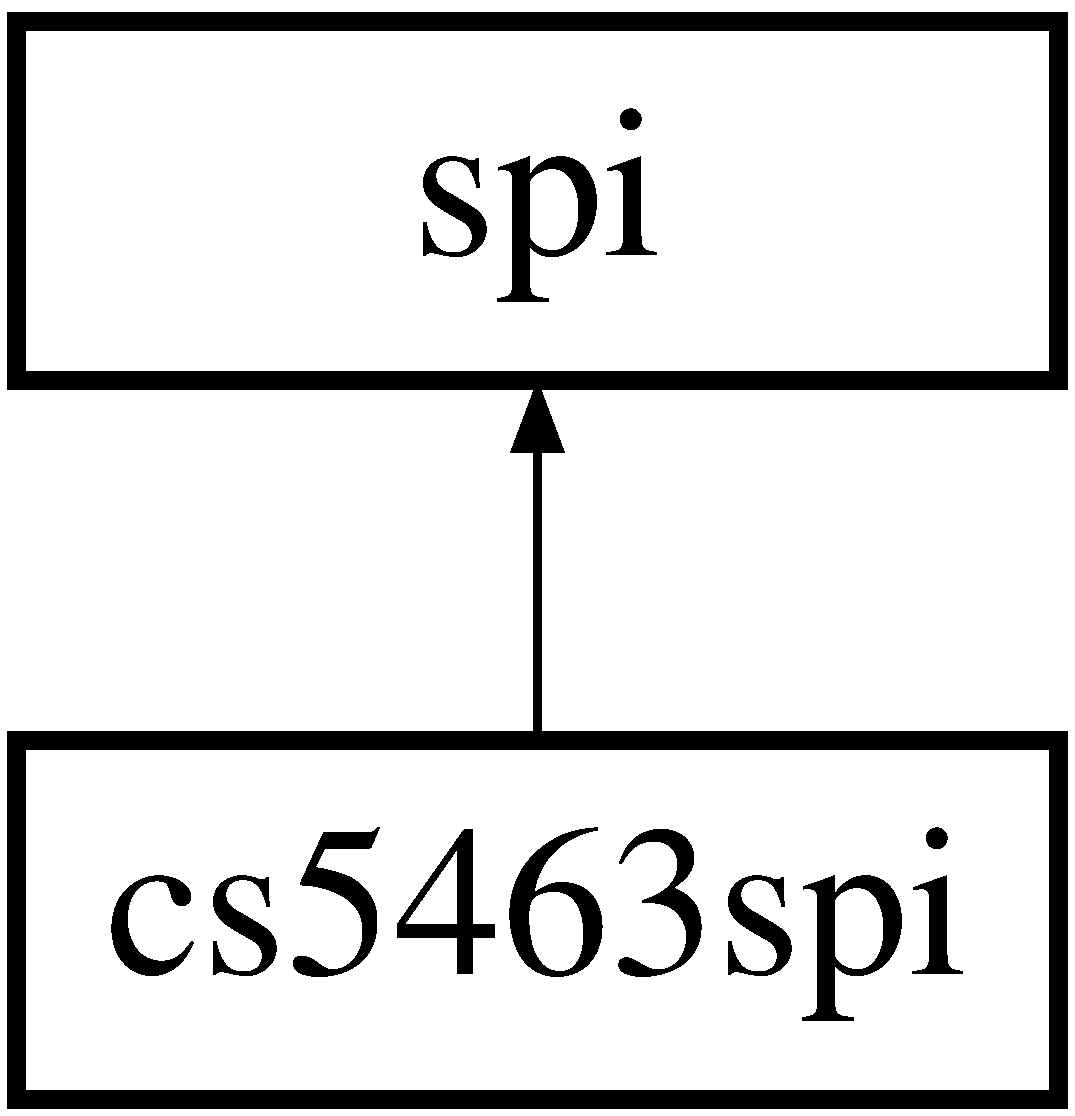
\includegraphics[height=2.000000cm]{classspi}
\end{center}
\end{figure}
\subsection*{Public Member Functions}
\begin{DoxyCompactItemize}
\item 
virtual \hyperlink{classspi_aa7039ccea879c1194360b401427f7b93}{$\sim$spi} ()
\item 
\hypertarget{classspi_a34b00f5bd260681619fee418239048a0}{virtual void {\bfseries Serial\-Port\-Init} ()}\label{classspi_a34b00f5bd260681619fee418239048a0}

\item 
\hypertarget{classspi_a94309b811b02a030d1a37eca9e27b286}{virtual void {\bfseries Read\-Values} ()}\label{classspi_a94309b811b02a030d1a37eca9e27b286}

\item 
\hypertarget{classspi_ab4c9b1d0f205e9dfac00107bc8fe1729}{virtual void {\bfseries Run} ()}\label{classspi_ab4c9b1d0f205e9dfac00107bc8fe1729}

\item 
\hypertarget{classspi_a1676554345a6127503f10d117f5b242d}{virtual bool {\bfseries Calibrate} (int cal\-Type)}\label{classspi_a1676554345a6127503f10d117f5b242d}

\item 
\hypertarget{classspi_ab5338399676761d03e503fa8f55ff4f6}{int {\bfseries open\-Device} (const char $\ast$p\-Device)}\label{classspi_ab5338399676761d03e503fa8f55ff4f6}

\item 
\hypertarget{classspi_af0e4702c999e07c9d2655cae8d12d1a4}{void {\bfseries set\-Spi\-Speed} (uint32\-\_\-t spi\-Speed)}\label{classspi_af0e4702c999e07c9d2655cae8d12d1a4}

\item 
\hypertarget{classspi_a24d0af0b21a8f58127d18c7cf77f0fd2}{void {\bfseries set\-Spi\-Delay} (uint16\-\_\-t spi\-Delay)}\label{classspi_a24d0af0b21a8f58127d18c7cf77f0fd2}

\item 
\hypertarget{classspi_aa81694fe53868e64ad9ef35e9003ac96}{void {\bfseries set\-Bit\-Order} (uint8\-\_\-t bit\-Order)}\label{classspi_aa81694fe53868e64ad9ef35e9003ac96}

\item 
\hypertarget{classspi_aa1251c2275e3a868291c85106de2f44b}{void {\bfseries set\-Log} (\hyperlink{classSystemLog}{System\-Log} $\ast$pspi\-Sys\-Log)}\label{classspi_aa1251c2275e3a868291c85106de2f44b}

\item 
\hypertarget{classspi_a868d26f2805f7a0a5ab2b45fef847a3d}{void {\bfseries set\-Logger} (\hyperlink{classLogger}{Logger} $\ast$my\-Logger)}\label{classspi_a868d26f2805f7a0a5ab2b45fef847a3d}

\item 
virtual void \hyperlink{classspi_af6b5a441ef9014df209fa3803d0fa68f}{spi\-Init} ()
\end{DoxyCompactItemize}
\subsection*{Protected Member Functions}
\begin{DoxyCompactItemize}
\item 
\hypertarget{classspi_a01ec3f79a14b29cee3fed591c477ecc4}{virtual void {\bfseries Write\-Register} ()}\label{classspi_a01ec3f79a14b29cee3fed591c477ecc4}

\item 
\hypertarget{classspi_ab82db7e47c0788f8593c0213688043cd}{virtual int {\bfseries Read\-Register} ()}\label{classspi_ab82db7e47c0788f8593c0213688043cd}

\item 
int \hyperlink{classspi_ace5d4b909ab9a103ae676df30db26836}{spi\-Send\-Receive} (uint8\-\_\-t $\ast$p\-Tx\-Buf, int i\-Tx\-Len, uint8\-\_\-t $\ast$p\-Rx\-Buf, int i\-Rx\-Len)
\item 
void \hyperlink{classspi_ab1569afd18aaa3ecaacc5252dab1177c}{spi\-Init\-Bit\-Order} ()
\item 
\hypertarget{classspi_a911578bfdd06fb5a4572069213072e53}{void {\bfseries set\-Spi\-Wr\-Mode} (uint8\-\_\-t spi\-Wr\-Mode)}\label{classspi_a911578bfdd06fb5a4572069213072e53}

\item 
\hypertarget{classspi_aea783dd071bb43a6cd05bc9cf4acb0d4}{void {\bfseries set\-Spi\-Rd\-Mode} (uint8\-\_\-t spi\-Rd\-Mode)}\label{classspi_aea783dd071bb43a6cd05bc9cf4acb0d4}

\item 
\hypertarget{classspi_aeb466902f0246e674230656c36260417}{void {\bfseries set\-Spi\-Mode} (uint8\-\_\-t spi\-Mode)}\label{classspi_aeb466902f0246e674230656c36260417}

\item 
\hypertarget{classspi_a0ca79e4dfeb0520519aae82576881229}{void {\bfseries set\-Spi\-B\-P\-W} (uint8\-\_\-t spi\-B\-P\-W)}\label{classspi_a0ca79e4dfeb0520519aae82576881229}

\item 
\hypertarget{classspi_a00c5efd63b774a1d50d3e69c8a49e0fa}{void {\bfseries set\-Spi\-Max\-Speed} (uint32\-\_\-t max\-Speed)}\label{classspi_a00c5efd63b774a1d50d3e69c8a49e0fa}

\item 
void \hyperlink{classspi_a71d243d92efaea106a3ee14970ea5ebe}{current\-Time\-Date} ()
\end{DoxyCompactItemize}
\subsection*{Protected Attributes}
\begin{DoxyCompactItemize}
\item 
\hypertarget{classspi_a30e62f162a7381cb154ceba749c3f9ba}{\hyperlink{classSystemLog}{System\-Log} $\ast$ {\bfseries m\-\_\-my\-S\-P\-I\-Sys\-Log}}\label{classspi_a30e62f162a7381cb154ceba749c3f9ba}

\item 
\hypertarget{classspi_a6b36076244edf6f661198f69c6b89b2d}{\hyperlink{classLogger}{Logger} $\ast$ {\bfseries m\-\_\-p\-My\-Logger}}\label{classspi_a6b36076244edf6f661198f69c6b89b2d}

\item 
\hypertarget{classspi_aa584b9b3ec842ac93204341966469d4c}{std\-::string {\bfseries m\-\_\-date\-Time}}\label{classspi_aa584b9b3ec842ac93204341966469d4c}

\end{DoxyCompactItemize}
\subsection*{Private Member Functions}
\begin{DoxyCompactItemize}
\item 
void \hyperlink{classspi_a7a176c5e112e2de900a823756d07af9d}{spi\-Abort} (const char $\ast$msg)
\item 
\hypertarget{classspi_a6855e6d729c1b70a51323596503b43a7}{{\bfseries spi} (const \hyperlink{classspi}{spi} \&)=delete}\label{classspi_a6855e6d729c1b70a51323596503b43a7}

\item 
\hypertarget{classspi_af6266e8c219e5b5ef4be205239379f14}{const \hyperlink{classspi}{spi} \& {\bfseries operator=} (const \hyperlink{classspi}{spi} \&)=delete}\label{classspi_af6266e8c219e5b5ef4be205239379f14}

\end{DoxyCompactItemize}
\subsection*{Private Attributes}
\begin{DoxyCompactItemize}
\item 
\hypertarget{classspi_afa6f0cf71472956e1b063b60421d6eeb}{\hyperlink{structspiParams}{spi\-Params} {\bfseries m\-\_\-spi\-Params}}\label{classspi_afa6f0cf71472956e1b063b60421d6eeb}

\end{DoxyCompactItemize}


\subsection{Detailed Description}
S\-P\-I is a abstract base class that defines the functionality of S\-P\-I. the clas is an S\-P\-I and has a Sys log member to write messages ang error to the linux sys log utility. 

\subsection{Constructor \& Destructor Documentation}
\hypertarget{classspi_aa7039ccea879c1194360b401427f7b93}{\index{spi@{spi}!$\sim$spi@{$\sim$spi}}
\index{$\sim$spi@{$\sim$spi}!spi@{spi}}
\subsubsection[{$\sim$spi}]{\setlength{\rightskip}{0pt plus 5cm}spi\-::$\sim$spi (
\begin{DoxyParamCaption}
{}
\end{DoxyParamCaption}
)\hspace{0.3cm}{\ttfamily [virtual]}}}\label{classspi_aa7039ccea879c1194360b401427f7b93}
Virtual destructor 

\subsection{Member Function Documentation}
\hypertarget{classspi_a71d243d92efaea106a3ee14970ea5ebe}{\index{spi@{spi}!current\-Time\-Date@{current\-Time\-Date}}
\index{current\-Time\-Date@{current\-Time\-Date}!spi@{spi}}
\subsubsection[{current\-Time\-Date}]{\setlength{\rightskip}{0pt plus 5cm}void spi\-::current\-Time\-Date (
\begin{DoxyParamCaption}
{}
\end{DoxyParamCaption}
)\hspace{0.3cm}{\ttfamily [protected]}}}\label{classspi_a71d243d92efaea106a3ee14970ea5ebe}
void Current\-Time\-Date() Works out the current date and time when sensor data was read. \hypertarget{classspi_a7a176c5e112e2de900a823756d07af9d}{\index{spi@{spi}!spi\-Abort@{spi\-Abort}}
\index{spi\-Abort@{spi\-Abort}!spi@{spi}}
\subsubsection[{spi\-Abort}]{\setlength{\rightskip}{0pt plus 5cm}void spi\-::spi\-Abort (
\begin{DoxyParamCaption}
\item[{const char $\ast$}]{msg}
\end{DoxyParamCaption}
)\hspace{0.3cm}{\ttfamily [private]}}}\label{classspi_a7a176c5e112e2de900a823756d07af9d}
Abort the application, but before it writes to the system log as an error. \hypertarget{classspi_af6b5a441ef9014df209fa3803d0fa68f}{\index{spi@{spi}!spi\-Init@{spi\-Init}}
\index{spi\-Init@{spi\-Init}!spi@{spi}}
\subsubsection[{spi\-Init}]{\setlength{\rightskip}{0pt plus 5cm}void spi\-::spi\-Init (
\begin{DoxyParamCaption}
{}
\end{DoxyParamCaption}
)\hspace{0.3cm}{\ttfamily [virtual]}}}\label{classspi_af6b5a441ef9014df209fa3803d0fa68f}
Initializes the spi driver 

Reimplemented in \hyperlink{classcs5463spi_ab61f5c633635597575dd756dd26391f3}{cs5463spi}.

\hypertarget{classspi_ab1569afd18aaa3ecaacc5252dab1177c}{\index{spi@{spi}!spi\-Init\-Bit\-Order@{spi\-Init\-Bit\-Order}}
\index{spi\-Init\-Bit\-Order@{spi\-Init\-Bit\-Order}!spi@{spi}}
\subsubsection[{spi\-Init\-Bit\-Order}]{\setlength{\rightskip}{0pt plus 5cm}void spi\-::spi\-Init\-Bit\-Order (
\begin{DoxyParamCaption}
{}
\end{DoxyParamCaption}
)\hspace{0.3cm}{\ttfamily [protected]}}}\label{classspi_ab1569afd18aaa3ecaacc5252dab1177c}
Sets bit order \hypertarget{classspi_ace5d4b909ab9a103ae676df30db26836}{\index{spi@{spi}!spi\-Send\-Receive@{spi\-Send\-Receive}}
\index{spi\-Send\-Receive@{spi\-Send\-Receive}!spi@{spi}}
\subsubsection[{spi\-Send\-Receive}]{\setlength{\rightskip}{0pt plus 5cm}int spi\-::spi\-Send\-Receive (
\begin{DoxyParamCaption}
\item[{uint8\-\_\-t $\ast$}]{p\-Tx\-Buf, }
\item[{int}]{i\-Tx\-Len, }
\item[{uint8\-\_\-t $\ast$}]{p\-Rx\-Buf, }
\item[{int}]{i\-Rx\-Len}
\end{DoxyParamCaption}
)\hspace{0.3cm}{\ttfamily [protected]}}}\label{classspi_ace5d4b909ab9a103ae676df30db26836}
spi\-Send\-Receive has two functionalities sends$\vert$/writes to the S\-P\-I and send/receive from the S\-P\-I. The method make use of the linux function ioctl that performs the generic I/\-O operations. 

The documentation for this class was generated from the following files\-:\begin{DoxyCompactItemize}
\item 
common/spi.\-h\item 
common/spi.\-cpp\end{DoxyCompactItemize}

\hypertarget{structspiParams}{\section{spi\-Params Struct Reference}
\label{structspiParams}\index{spi\-Params@{spi\-Params}}
}
\subsection*{Data Fields}
\begin{DoxyCompactItemize}
\item 
\hypertarget{structspiParams_a943b444e77f506b67c26334326be4caf}{uint8\-\_\-t {\bfseries bit\-Order}}\label{structspiParams_a943b444e77f506b67c26334326be4caf}

\item 
\hypertarget{structspiParams_abf2bae4035ced0c45ced2618c2150d66}{uint8\-\_\-t {\bfseries spi\-Wr\-Mode}}\label{structspiParams_abf2bae4035ced0c45ced2618c2150d66}

\item 
\hypertarget{structspiParams_a24ce28ae11d13edb3cc2611790f74448}{uint8\-\_\-t {\bfseries spi\-Rd\-Mode}}\label{structspiParams_a24ce28ae11d13edb3cc2611790f74448}

\item 
\hypertarget{structspiParams_adfa9ae8f40748929cd125f2a2627a490}{uint8\-\_\-t {\bfseries spi\-B\-P\-W}}\label{structspiParams_adfa9ae8f40748929cd125f2a2627a490}

\item 
\hypertarget{structspiParams_a29a2a33adc949277f980d55c573bcb07}{uint32\-\_\-t {\bfseries spi\-Speed}}\label{structspiParams_a29a2a33adc949277f980d55c573bcb07}

\item 
\hypertarget{structspiParams_ac6af66e49fb2c4f84b4fd09e7f2df147}{uint32\-\_\-t {\bfseries spi\-Max\-Speed}}\label{structspiParams_ac6af66e49fb2c4f84b4fd09e7f2df147}

\item 
\hypertarget{structspiParams_a7d276b4bdd88c78495a6d87919ea9664}{uint16\-\_\-t {\bfseries spi\-Delay}}\label{structspiParams_a7d276b4bdd88c78495a6d87919ea9664}

\item 
\hypertarget{structspiParams_a75dcaec546d7e6c605f854871b6cf2ca}{int {\bfseries fd}}\label{structspiParams_a75dcaec546d7e6c605f854871b6cf2ca}

\end{DoxyCompactItemize}
\subsection*{Static Public Attributes}
\begin{DoxyCompactItemize}
\item 
\hypertarget{structspiParams_a6f2ed69ae1dc110d7cd3de5e6b145a94}{static const char $\ast$ {\bfseries device}}\label{structspiParams_a6f2ed69ae1dc110d7cd3de5e6b145a94}

\end{DoxyCompactItemize}


The documentation for this struct was generated from the following file\-:\begin{DoxyCompactItemize}
\item 
common/spi.\-h\end{DoxyCompactItemize}

\hypertarget{classSystemLog}{\section{System\-Log Class Reference}
\label{classSystemLog}\index{System\-Log@{System\-Log}}
}
\subsection*{Public Member Functions}
\begin{DoxyCompactItemize}
\item 
\hypertarget{classSystemLog_a95cdee97db2f439dc68408f7428a032e}{{\bfseries System\-Log} (const char $\ast$p\-Daemon)}\label{classSystemLog_a95cdee97db2f439dc68408f7428a032e}

\item 
\hypertarget{classSystemLog_a8aad2362d938a8973dc2d06bb1465415}{void {\bfseries write\-Msg\-Log} (const char $\ast$msg)}\label{classSystemLog_a8aad2362d938a8973dc2d06bb1465415}

\item 
\hypertarget{classSystemLog_a394f7593601ae73851cff8e7fc6cd299}{int {\bfseries write\-Err\-Log} (const char $\ast$msg)}\label{classSystemLog_a394f7593601ae73851cff8e7fc6cd299}

\end{DoxyCompactItemize}
\subsection*{Private Attributes}
\begin{DoxyCompactItemize}
\item 
\hypertarget{classSystemLog_a169a179640dec0f42020352a8a56f798}{const char $\ast$ {\bfseries m\-\_\-p\-Deamon}}\label{classSystemLog_a169a179640dec0f42020352a8a56f798}

\end{DoxyCompactItemize}


The documentation for this class was generated from the following files\-:\begin{DoxyCompactItemize}
\item 
common/System\-Log.\-h\item 
common/System\-Log.\-cpp\end{DoxyCompactItemize}

\hypertarget{structtimeDate}{\section{time\-Date Struct Reference}
\label{structtimeDate}\index{time\-Date@{time\-Date}}
}
\subsection*{Data Fields}
\begin{DoxyCompactItemize}
\item 
\hypertarget{structtimeDate_a4513a3b33d516596a3270a42889d1d77}{std\-::time\-\_\-t {\bfseries time}}\label{structtimeDate_a4513a3b33d516596a3270a42889d1d77}

\item 
\hypertarget{structtimeDate_aba1a6fdf27de686648a1576d29833a9a}{std\-::string {\bfseries date}}\label{structtimeDate_aba1a6fdf27de686648a1576d29833a9a}

\end{DoxyCompactItemize}


The documentation for this struct was generated from the following file\-:\begin{DoxyCompactItemize}
\item 
common/spi.\-h\end{DoxyCompactItemize}

%--- End generated contents ---

% Index
\newpage
\phantomsection
\addcontentsline{toc}{chapter}{Index}
\printindex

\end{document}
